% !TEX program = lualatex
\documentclass[11pt]{article}
\usepackage[utf8]{inputenc}
\usepackage{graphicx}
\usepackage{amsmath}
\usepackage{hyperref}
\usepackage{caption}
\usepackage{subcaption}
\usepackage{geometry}
\usepackage{float}
\usepackage{pdfpages}
\usepackage{pifont}
\usepackage{todonotes}
\usepackage{booktabs}
\usepackage{array}
\usepackage{xcolor}
\usepackage{colortbl}
\usepackage{enumitem}
\usepackage{setspace}
\usepackage{url}
\usepackage{tikz}
\usetikzlibrary{positioning}
\usepackage{titlesec}
\titleformat{\paragraph}
  {\normalfont\bfseries}{\theparagraph}{1em}{}
\titlespacing*{\paragraph}
  {0pt}{2.5ex plus 1ex minus .2ex}{0.8ex}


\geometry{margin=2.5cm}
\sloppy
\onehalfspacing


\title{CreaRobot}
\author{Marco Grandclaude}
\date{\today}

\begin{document}

\begin{titlepage}
    \centering

    \centering
    % Logos
    \begin{minipage}{0.45\textwidth}
        
\includegraphics[height=2cm]{figures/logo_sorbonne.png}\\[0.3cm]
        
\includegraphics[height=2cm]{figures/logo_polytech.png}
    \end{minipage}
    \hfill
    \begin{minipage}{0.45\textwidth}
        \raggedleft
        
\includegraphics[height=2cm]{figures/logo_lutin.png}
    \end{minipage}

    \vspace{1cm}

    % Title
    {\Huge \textbf{CreaRobot}} \\[0.5cm]
    {\Large Rapport de Stage de Fin d'études} \\[1cm]

    % Info autor
    {\Large Marco Grandclaude} \\[0.3cm]
    {\large Sorbonne Université – Polytech Sorbonne} \\[0.2cm]
    {\large Robotique} \\[0.2cm]
    {\large 2025–2026} \\[1cm]

    % Info Stage
    {\large 1er mars, 2026 – 31 août, 2026} \\[0.3cm]
    {\large Lutin - Laboratoire CHART} \\[1cm]

    % Photo de couverture
    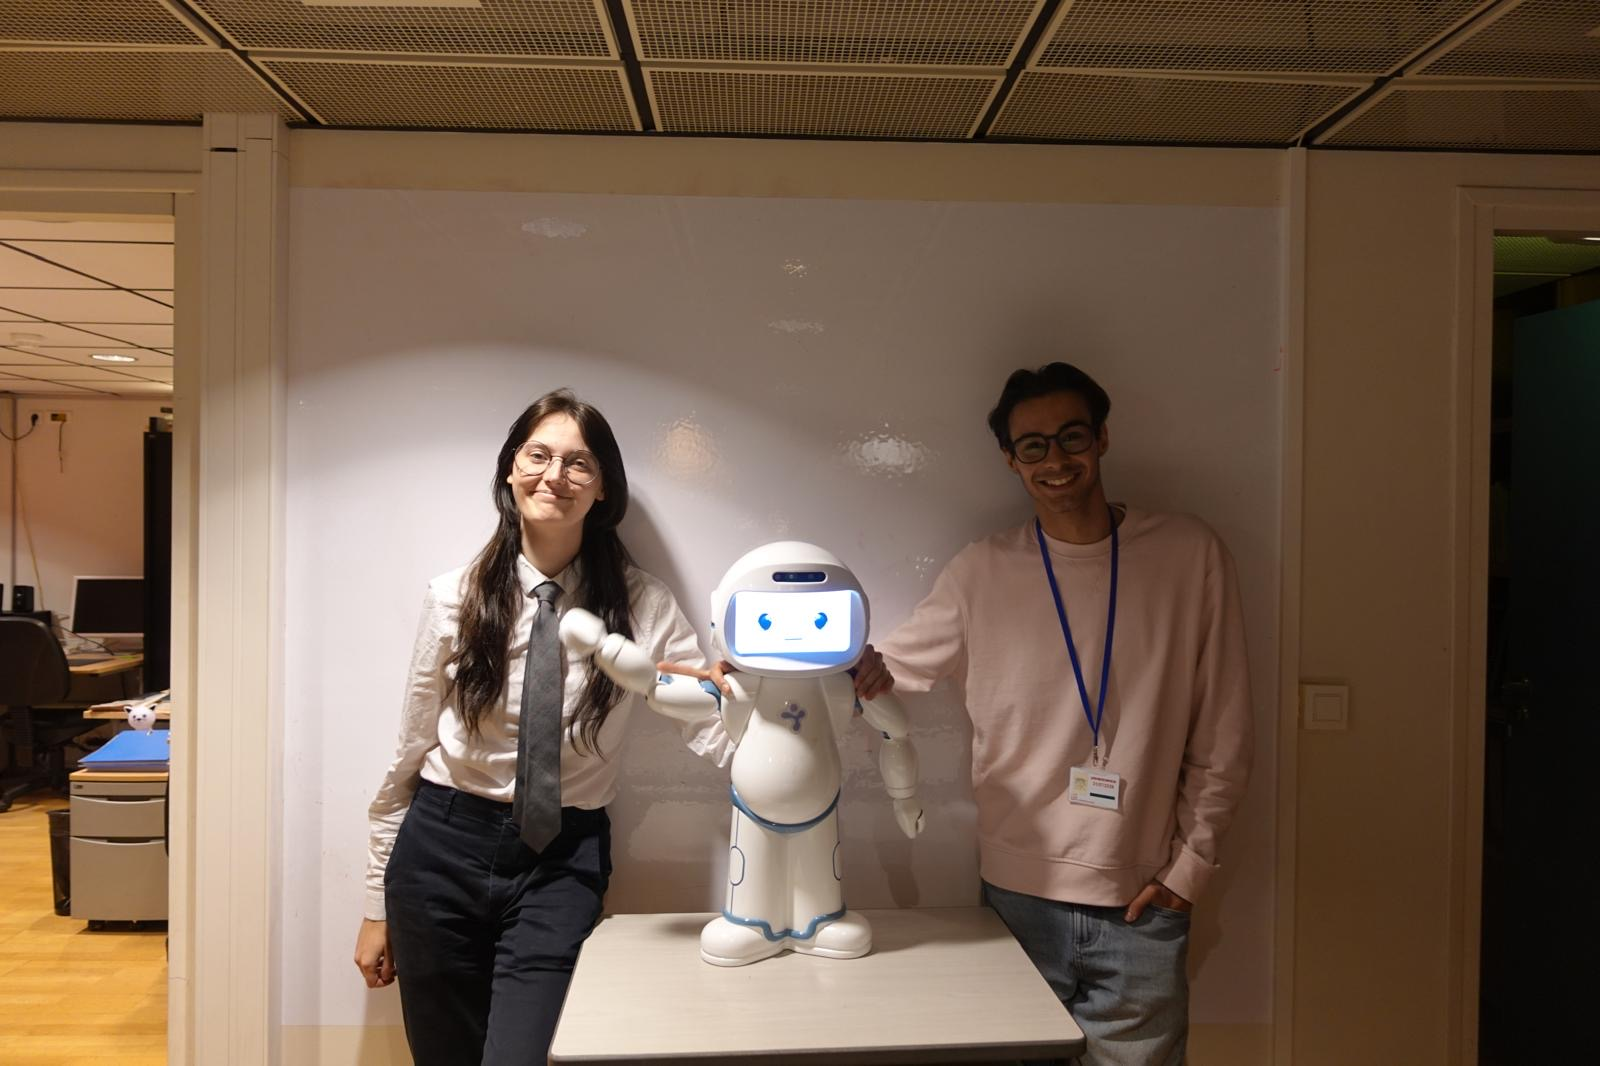
\includegraphics[width=0.6\textwidth]{figures/lutin_intro.jpg}

    % Bottom
    \vfill
    {\large Paris, \today}
\end{titlepage}
\newpage

\pagenumbering{gobble}

% Abstract
\begin{center}
    \Huge \textbf{Abstract}
\end{center}
\vspace{0.5cm}
\newpage

% Acknowledgments
\begin{center}
    \Huge \textbf{Remerciements}
\end{center}
\vspace{0.5cm}
Je tiens à remercier sincèrement ma famille, mes parents, mes frères et ma sœur pour leur soutien tout au long de mes études et de ce stage.

Je remercie également mon tuteur académique, Mahdi Khoramshahi, pour son implication dans le suivi de ce projet et pour avoir assuré le cadre pédagogique de ce travail de recherche.

Ma profonde gratitude s'adresse à mon maître de stage, Salvatore Anzalone, pour son mentorat, ses précieux conseils et l'accompagnement constant qu'il m'a apporté tout au long de cette expérience.

Je tiens à adresser un merci tout particulier à Claudie Cuveillier pour notre collaboration au sein de ce partenariat. Son travail sur la dimension sciences cognitives a été fondamental pour la réussite du projet et je la remercie pour cette synergie extrêmement productive.

Je souhaite aussi remercier Geoffrey Tissier, responsable technique de la plateforme, pour son aide précieuse, ainsi que les doctorants et les autres stagiaires pour nos échanges enrichissants et la collaboration qui a rendu ce stage très agréable.

Enfin, je remercie le laboratoire pour son accueil et pour m'avoir permis d'évoluer au sein d'un environnement scientifique aussi stimulant et propice à l'innovation.
\newpage

\tableofcontents
\newpage
\pagenumbering{arabic}

\listoffigures
\newpage
\listoftables
\newpage

% ============================================================
\section{Introduction}

\subsection{Vue d'ensemble de la problématique}

La créativité est une compétence clé du développement de l'enfant, à la fois pour la construction cognitive et l'expression de soi \cite{fasko2001}. En contexte scolaire, un des freins récurrents à son développement est le manque d'outils capables d'apporter un retour individualisé et en temps réel sur une production créative \cite{cremin2021} ; un enseignant ne peut matériellement pas suivre en continu la démarche créative de chaque enfant.

Les robots sociaux sont déjà utilisés depuis plusieurs années pour accompagner les apprentissages des enfants, notamment parce qu'ils peuvent agir comme des agents qui suscitent la créativité par démonstration et étayage \cite{ali2021}. Face à un participant, un robot peut aussi bien jouer un rôle de coach, en orientant et en stimulant son processus créatif, que de collègue, en contribuant lui-même activement à la production \cite{lubart2005}. Ce qui change aujourd'hui, c'est que l'intelligence artificielle générative (GenAI, de l'anglais generative AI) permet à ce type de robot de produire un feedback beaucoup plus riche et contextualisé qu'auparavant : plusieurs travaux montrent qu'elle est désormais capable de produire des contenus créatifs comparables à ceux d'un humain \cite{haase2023}. La littérature reste cependant prudente sur son usage : mal employée, elle risque d'homogénéiser les idées produites et de réduire la nouveauté à l'échelle collective \cite{doshi2024}. C'est pour répondre à cette tension que Vinchon, Lubart et leurs collègues défendent un scénario de collaboration humain-IA de type "Co-Cre-AI-tion", où l'humain garde la main sur le processus créatif tout en étant assisté par l'IA \cite{vinchon2023} ; c'est cet équilibre que CreaRobot cherche à mettre en pratique à travers un robot, plutôt qu'à travers une IA seule et désincarnée.

Pour étudier cette interaction, la tâche de dessin est particulièrement adaptée : elle est accessible quel que soit l'âge ou le niveau du participant, intrinsèquement visuelle, donc directement perceptible par une caméra, et mesurable grâce à des instruments validés comme le Test for Creative Thinking – Drawing Production \cite{urban2005}.

C'est dans ce contexte que s'inscrit le projet CreaRobot, qui étudie l'utilisation d'un robot social équipé d'un modèle vision-langage pour améliorer la valeur du produit créatif dans une tâche de dessin. Ce travail a d'ailleurs donné lieu à une publication acceptée à ICMI Companion 2026 \cite{cuveillier2026crearobot}.

\subsection{Contexte scientifique}
% Note : garder cette partie concise, pas le cœur du rapport technique.

\subsubsection{Robotique sociale et interaction homme-robot}

Un robot social se distingue d'un robot industriel ou fonctionnel par sa capacité à interagir socialement avec l'humain, en s'appuyant sur des signaux comme le regard, la voix, les gestes ou les expressions faciales pour établir une relation \cite{breazeal2004}. Cette incarnation physique joue un rôle important dans l'interaction : un robot présent dans l'espace physique de l'utilisateur suscite un engagement plus fort qu'un agent virtuel affiché sur un écran ; un effet particulièrement marqué chez les enfants. Les robots sociaux sont ainsi déjà utilisés dans plusieurs domaines d'application, notamment l'éducation, où leur usage pour accompagner les apprentissages fait l'objet d'une littérature de plus en plus fournie \cite{belpaeme2018,johal2020}. C'est dans ce cadre que s'inscrit la créativité comme terrain d'application étudié dans ce rapport, présenté dans la partie suivante.

\subsubsection{La créativité et le test TCT-DP}

La créativité peut se définir comme la capacité à produire quelque chose à la fois nouveau, donc original, et adapté au contexte dans lequel il est produit, donc pertinent \cite{lubart2003}. Cette double exigence rend son évaluation délicate, en particulier dans une tâche graphique ouverte comme celle proposée dans ce projet, où il n'existe pas de bonne ou de mauvaise réponse. C'est pour répondre à cette difficulté que le TCT-DP a été conçu : un instrument dont la validité pour évaluer la créativité à partir d'une production graphique a été établie et largement reprise depuis \cite{urbanjellen1996,urban2005}. Le test lui-même, ainsi que ses critères de cotation, sont détaillés dans la partie Méthode (section~\ref{sec:protocole}).

\subsubsection{État de l'art : robots sociaux dans des protocoles expérimentaux}

Lorsque la production ne relève plus d'un seul créateur mais d'une collaboration entre un humain et un système computationnel, on parle de co-création, ou de co-créativité humain-machine. Kantosalo et Takala \cite{kantosalo2020} la définissent à travers un modèle dit des « cinq C » : un \textit{collectif}, formé d'un humain et d'une intelligence artificielle, \textit{collabore} pour produire une \textit{contribution} destinée à une \textit{communauté}, dans un \textit{contexte} donné. Cette lecture correspond directement à la situation visée par CreaRobot, où le participant et le robot forment un collectif produisant ensemble un dessin.

Pour qu'un tel collectif fonctionne, encore faut-il que le robot soit perçu par le participant comme un véritable partenaire d'interaction et non comme un simple outil. Cette perception repose en partie sur l'anthropomorphisme, c'est-à-dire l'attribution de traits humains au robot, qui le rend plus familier et plus prévisible aux yeux de l'utilisateur ; la littérature montre toutefois que ce levier ne favorise l'acceptation du robot qu'à condition que le participant conserve un sentiment de contrôle sur l'interaction elle-même \cite{david2026}.

La conception du comportement du robot doit par ailleurs composer avec une limite connue des outils génératifs : ceux-ci tendent spontanément vers la substitution plutôt que vers le soutien, en produisant à la place de l'utilisateur plutôt qu'avec lui \cite{lubart2003}. Cette tendance est renforcée par le comportement par défaut des grands modèles de langage, entraînés pour endosser un persona d'assistant serviable qui les pousse soit à acquiescer aux propositions de l'utilisateur, soit à prendre en charge la tâche à sa place \cite{lu2026} ; des travaux récents montrent qu'un pilotage plus structuré du dialogue permet de contraindre ce comportement par défaut \cite{galland2025}. Dans un contexte de co-création, la qualité d'un retour dépend également de sa nature : Rezwana et Ford \cite{rezwana2025} distinguent les suggestions divergentes, qui élargissent l'espace des possibles créatifs, des suggestions convergentes, plus adaptées aux phases de finalisation. Ces constats rejoignent la logique du prompt utilisé par le robot en condition C1, décrite en section~\ref{sec:condition_c1}.

\subsection{Le projet CreaRobot : question de recherche et enjeux}

Le projet CreaRobot pose une question de recherche centrale : un robot social peut-il, par
l'interaction, améliorer la créativité d'une personne en train de dessiner ?

Pour répondre à cette question, l'expérience repose sur le test de créativité TCT-DP
(Test for Creative Thinking – Drawing Production) \cite{urban2005}, un test standardisé
consistant à compléter une figure géométrique partielle. Le protocole compare trois conditions
expérimentales : un feedback neutre délivré par le robot (condition de contrôle), un échange piloté par un modèle de langage mêlant questions, suggestions et idées portant sur le dessin du participant (condition C1), et un retour visuel génératif projeté
sur la zone de dessin (condition C2).

L'enjeu technique de ce stage est de concevoir et développer de A à Z le système logiciel
permettant au robot social QTRobot (plateforme ROS\,1 / Python\,2.7), illustré en figure~\ref{fig:qtrobot},
d'interagir en temps réel avec des participants humains, en s'appuyant sur une intelligence déportée
sur un PC externe (ROS\,2 / Python\,3) : reconnaissance vocale, traitement du langage naturel, pilotage
des expressions et des gestes, synchronisation avec les phases du protocole.

\begin{figure}[H]
    \centering
    \vspace{0.3cm}
    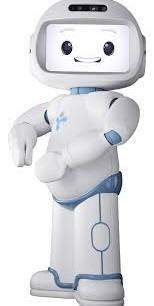
\includegraphics[height=10cm]{figures/qtrobot.jpeg}
    \caption{Le robot social QTRobot.}
    \label{fig:qtrobot}
\end{figure}

Le système a fait l'objet d'une première passation préliminaire, à visée exploratoire, lors de
la Semaine de la Science Infuse en avril 2026. La passation principale est quant à elle prévue
en octobre/novembre 2026.

\subsection{Contexte du stage, laboratoire CHART et plateforme Lutin}

\subsubsection{Contexte du stage}

Ce rapport présente le travail réalisé dans le cadre d'un stage technique effectué au sein du
laboratoire CHART, sur la plateforme Lutin, du 1\textsuperscript{er} mars 2025 au 31 août 2026.
Ce stage s'inscrit dans le cursus ingénieur de la filière Robotique de Polytech Sorbonne
(Sorbonne Université), en troisième année de cycle ingénieur.

Le stage a été encadré par Salvatore Anzalone, maître de stage, chercheur à CHART et directeur
de la plateforme Lutin, ainsi que par Mahdi Khoramshahi, tuteur académique à Polytech Sorbonne.
Le travail a été mené en collaboration étroite avec Claudie Cuveillier, stagiaire en ergonomie, qui a notamment pris en charge la conception des protocoles de dialogue pour le robot.

\subsubsection{Le laboratoire CHART et la plateforme Lutin}

Le laboratoire CHART (Cognitions Humaines et Artificielles) est une unité mixte de recherche.
Ses travaux portent sur les interactions entre cognition humaine et systèmes numériques, à
l'interface de la psychologie cognitive, des sciences de l'éducation et de l'intelligence
artificielle.

La plateforme Lutin est rattachée au laboratoire CHART et constitue son infrastructure expérimentale.
Le LUTIN (Laboratoire des Usages en Technologies d'Information Numériques) contrairement à
ce que son nom indique n’est pas un laboratoire mais est une plateforme de recherche collaborative
et pluridisciplinaire dédiée à l'étude des sciences cognitives et de la robotique, dont l'ambition
est d'explorer la relation entre l'humain et le numérique dans le cadre académique mais aussi industriel.
C'est un endroit où l'on étudie comment les gens utilisent les technologies, pour mieux les concevoir, les évaluer et,
in fine, les mettre au service des utilisateurs.
Le LUTIN est dirigé par Salvatore Anzalone, avec Ugo Ballenghein en tant que directeur adjoint,
tous deux membres du laboratoire CHArt.
Le LUTIN vise à développer des connaissances et des méthodes dans le champ des usages et des pratiques numériques, quels qu’en soient les domaines d’application. Pour ce faire, il dispose d’un parc d’équipements technologiques permettant l’analyse de mesures comportementales et neurophysiologiques en temps réel : eye-tracking, EEG, motion capture, réalité virtuelle, robotique ou encore dispositif de vitres sans tain pour observer les potentiels participants dans des cadres écologiques. Ces outils permettent d’aller bien au-delà du simple questionnaire et d’investiguer au mieux les comportements réels des utilisateurs face à une technologie.

\newpage

% ============================================================
\section{Méthode}

\subsection{L'expérience dans son ensemble}
\label{sec:protocole}
% Placé en tête de la Méthode pour donner au lecteur le contexte
% qui justifie chaque choix technique développé ensuite.

\subsubsection{Description du test de créativité TCT-DP}
\label{sec:tctdp_description}

Le TCT-DP (Test for Creative Thinking – Drawing Production) se présente sous la forme d'une feuille sur laquelle est imprimé un cadre carré fermé. À l'intérieur de ce cadre sont disposés cinq fragments graphiques simples et non reliés entre eux : une ligne courbe, un angle, un point isolé, un demi-cercle, et trois tirets alignés. Un sixième fragment se trouve en dehors du cadre : un petit carré ouvert. Il est demandé au participant de compléter le dessin comme il le souhaite, dans un temps limité. C'est un test standardisé et validé \cite{urban2005}, pensé pour être réalisé rapidement, y compris par des personnes qui ne dessinent pas habituellement.

Le test existe en deux versions, A et B, qui reprennent les six mêmes fragments mais selon une disposition inversée à 180 degrés l'une par rapport à l'autre (figure~\ref{fig:test_sheet}). Cette double version permet de contrebalancer l'effet que pourrait avoir la position d'un fragment sur la feuille sur la façon dont il est complété, plutôt que de laisser un même sens d'impression à chaque participant.

\begin{figure}[H]
    \centering
    \begin{subfigure}[b]{0.48\textwidth}
        \centering
        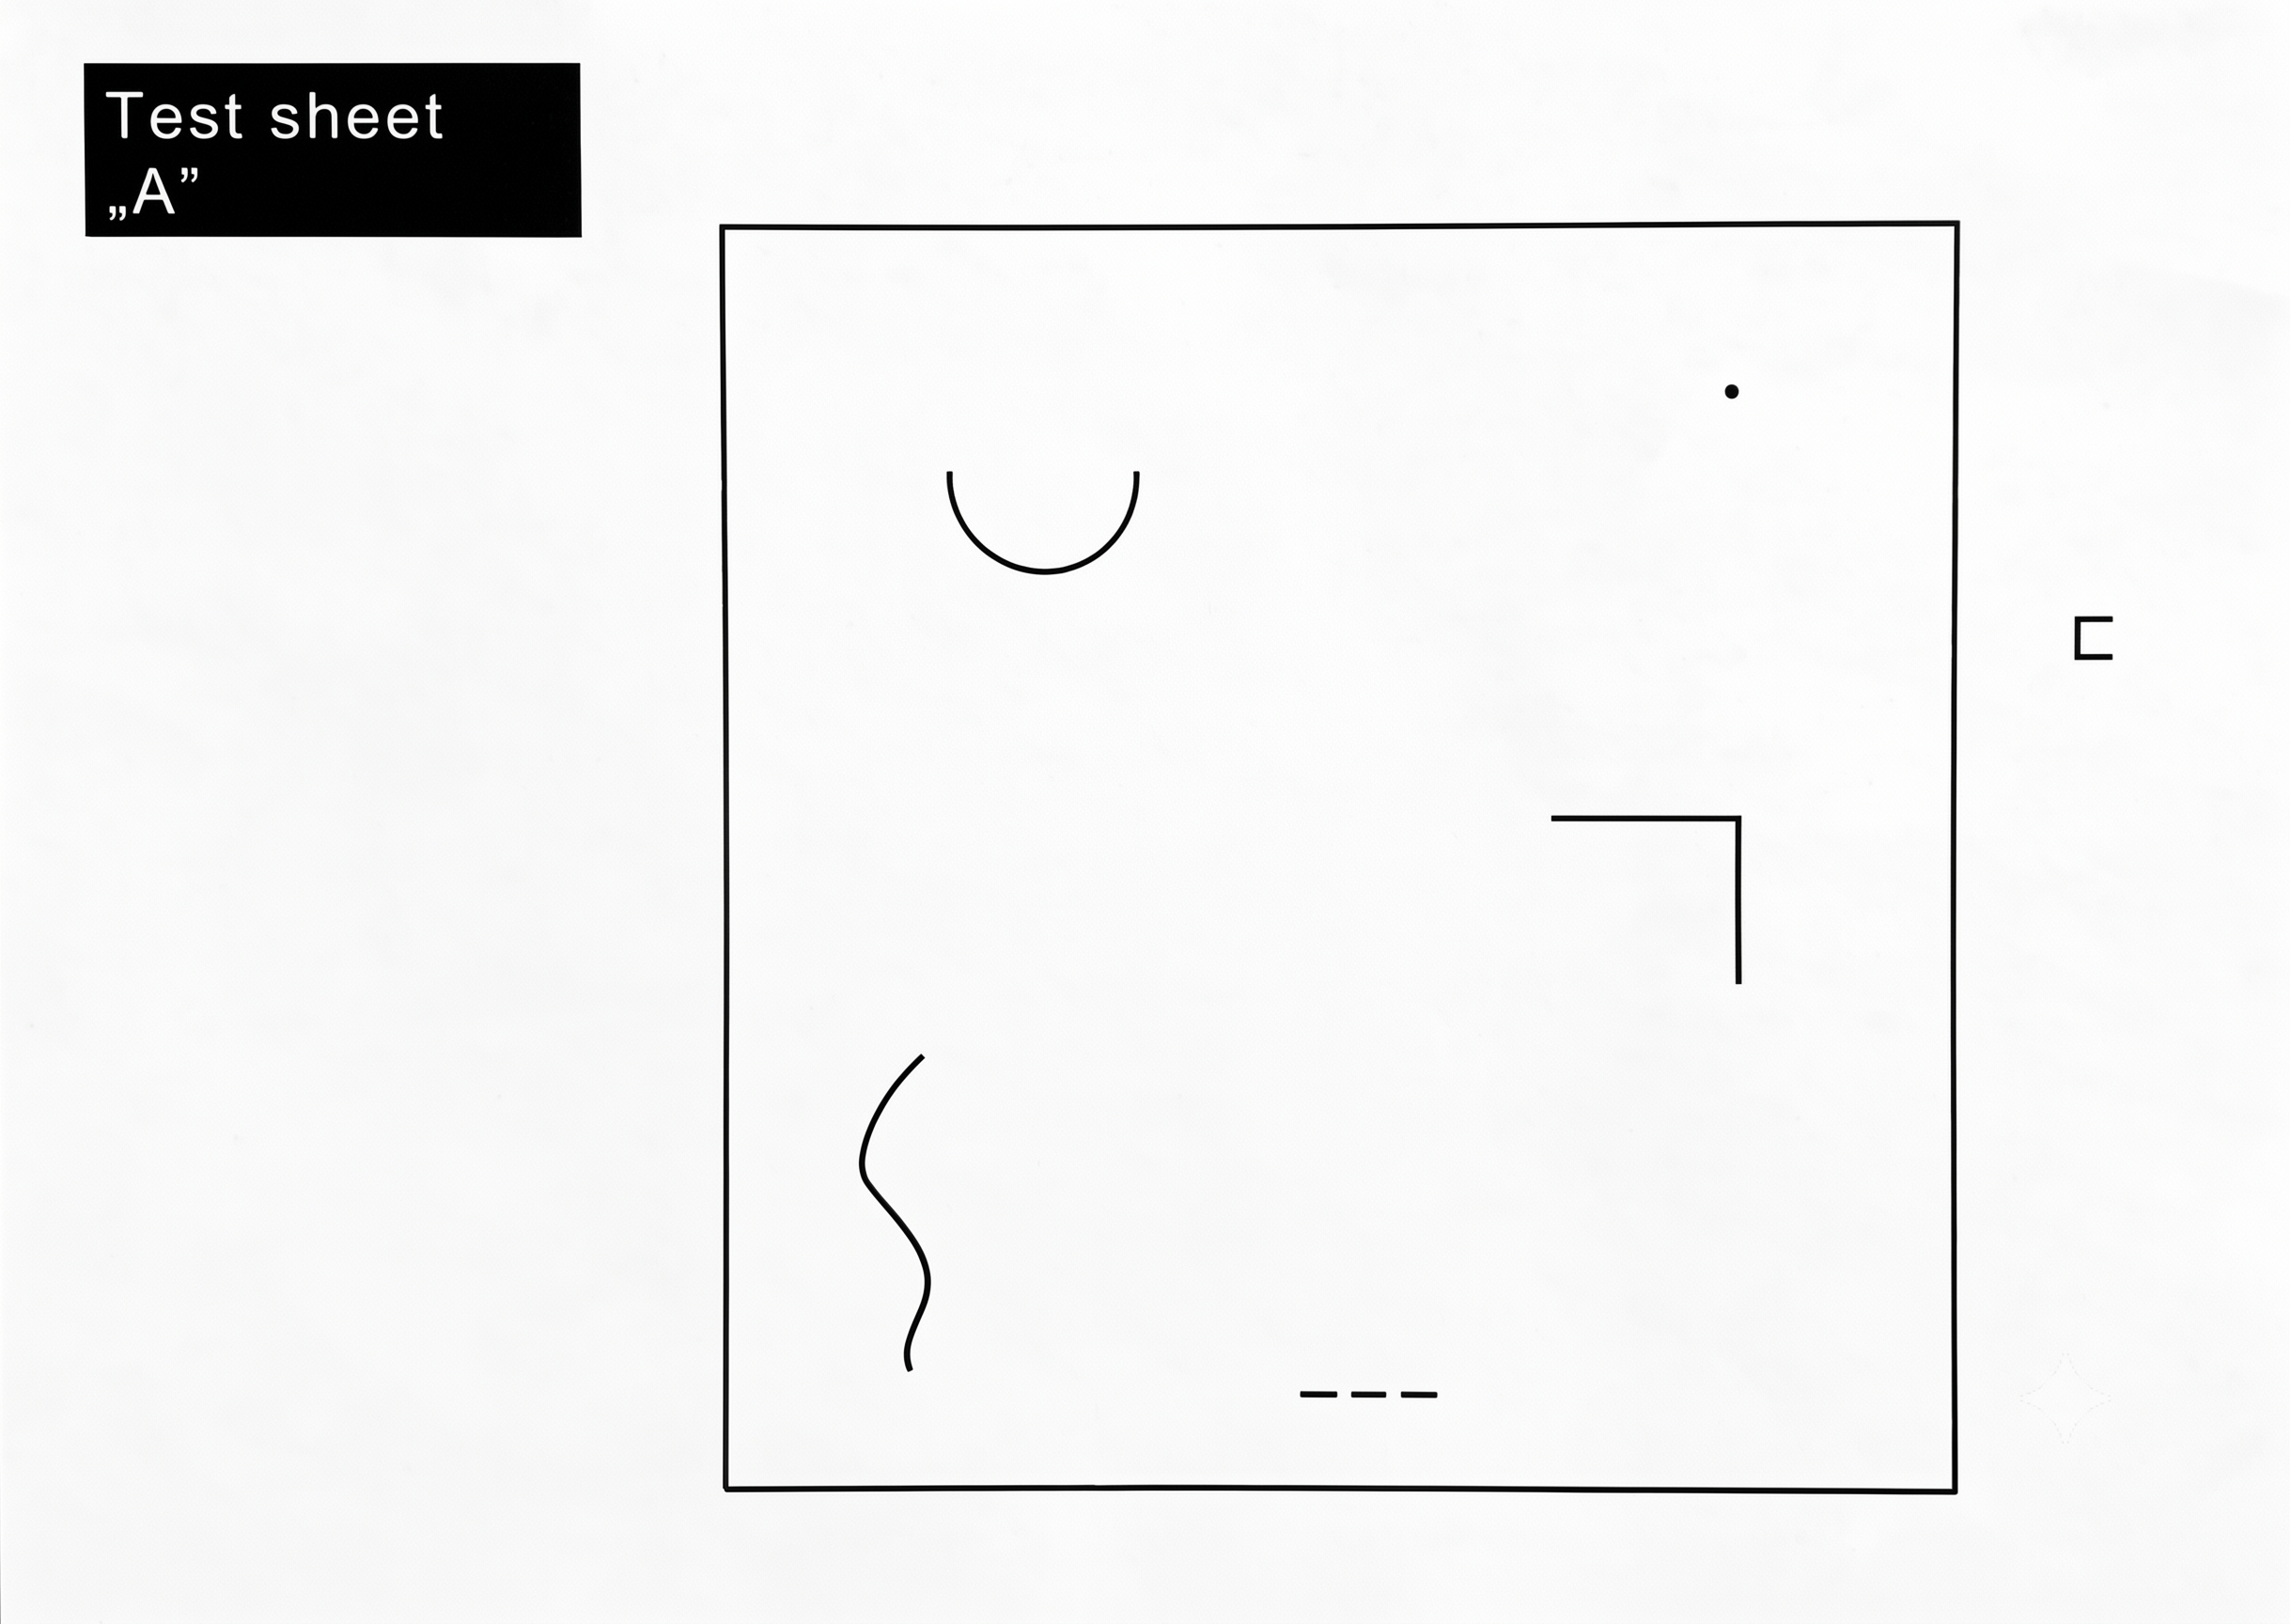
\includegraphics[width=\textwidth]{figures/test_sheet_A.png}
        \caption{Version A}
        \label{fig:test_sheet_a}
    \end{subfigure}
    \hfill
    \begin{subfigure}[b]{0.48\textwidth}
        \centering
        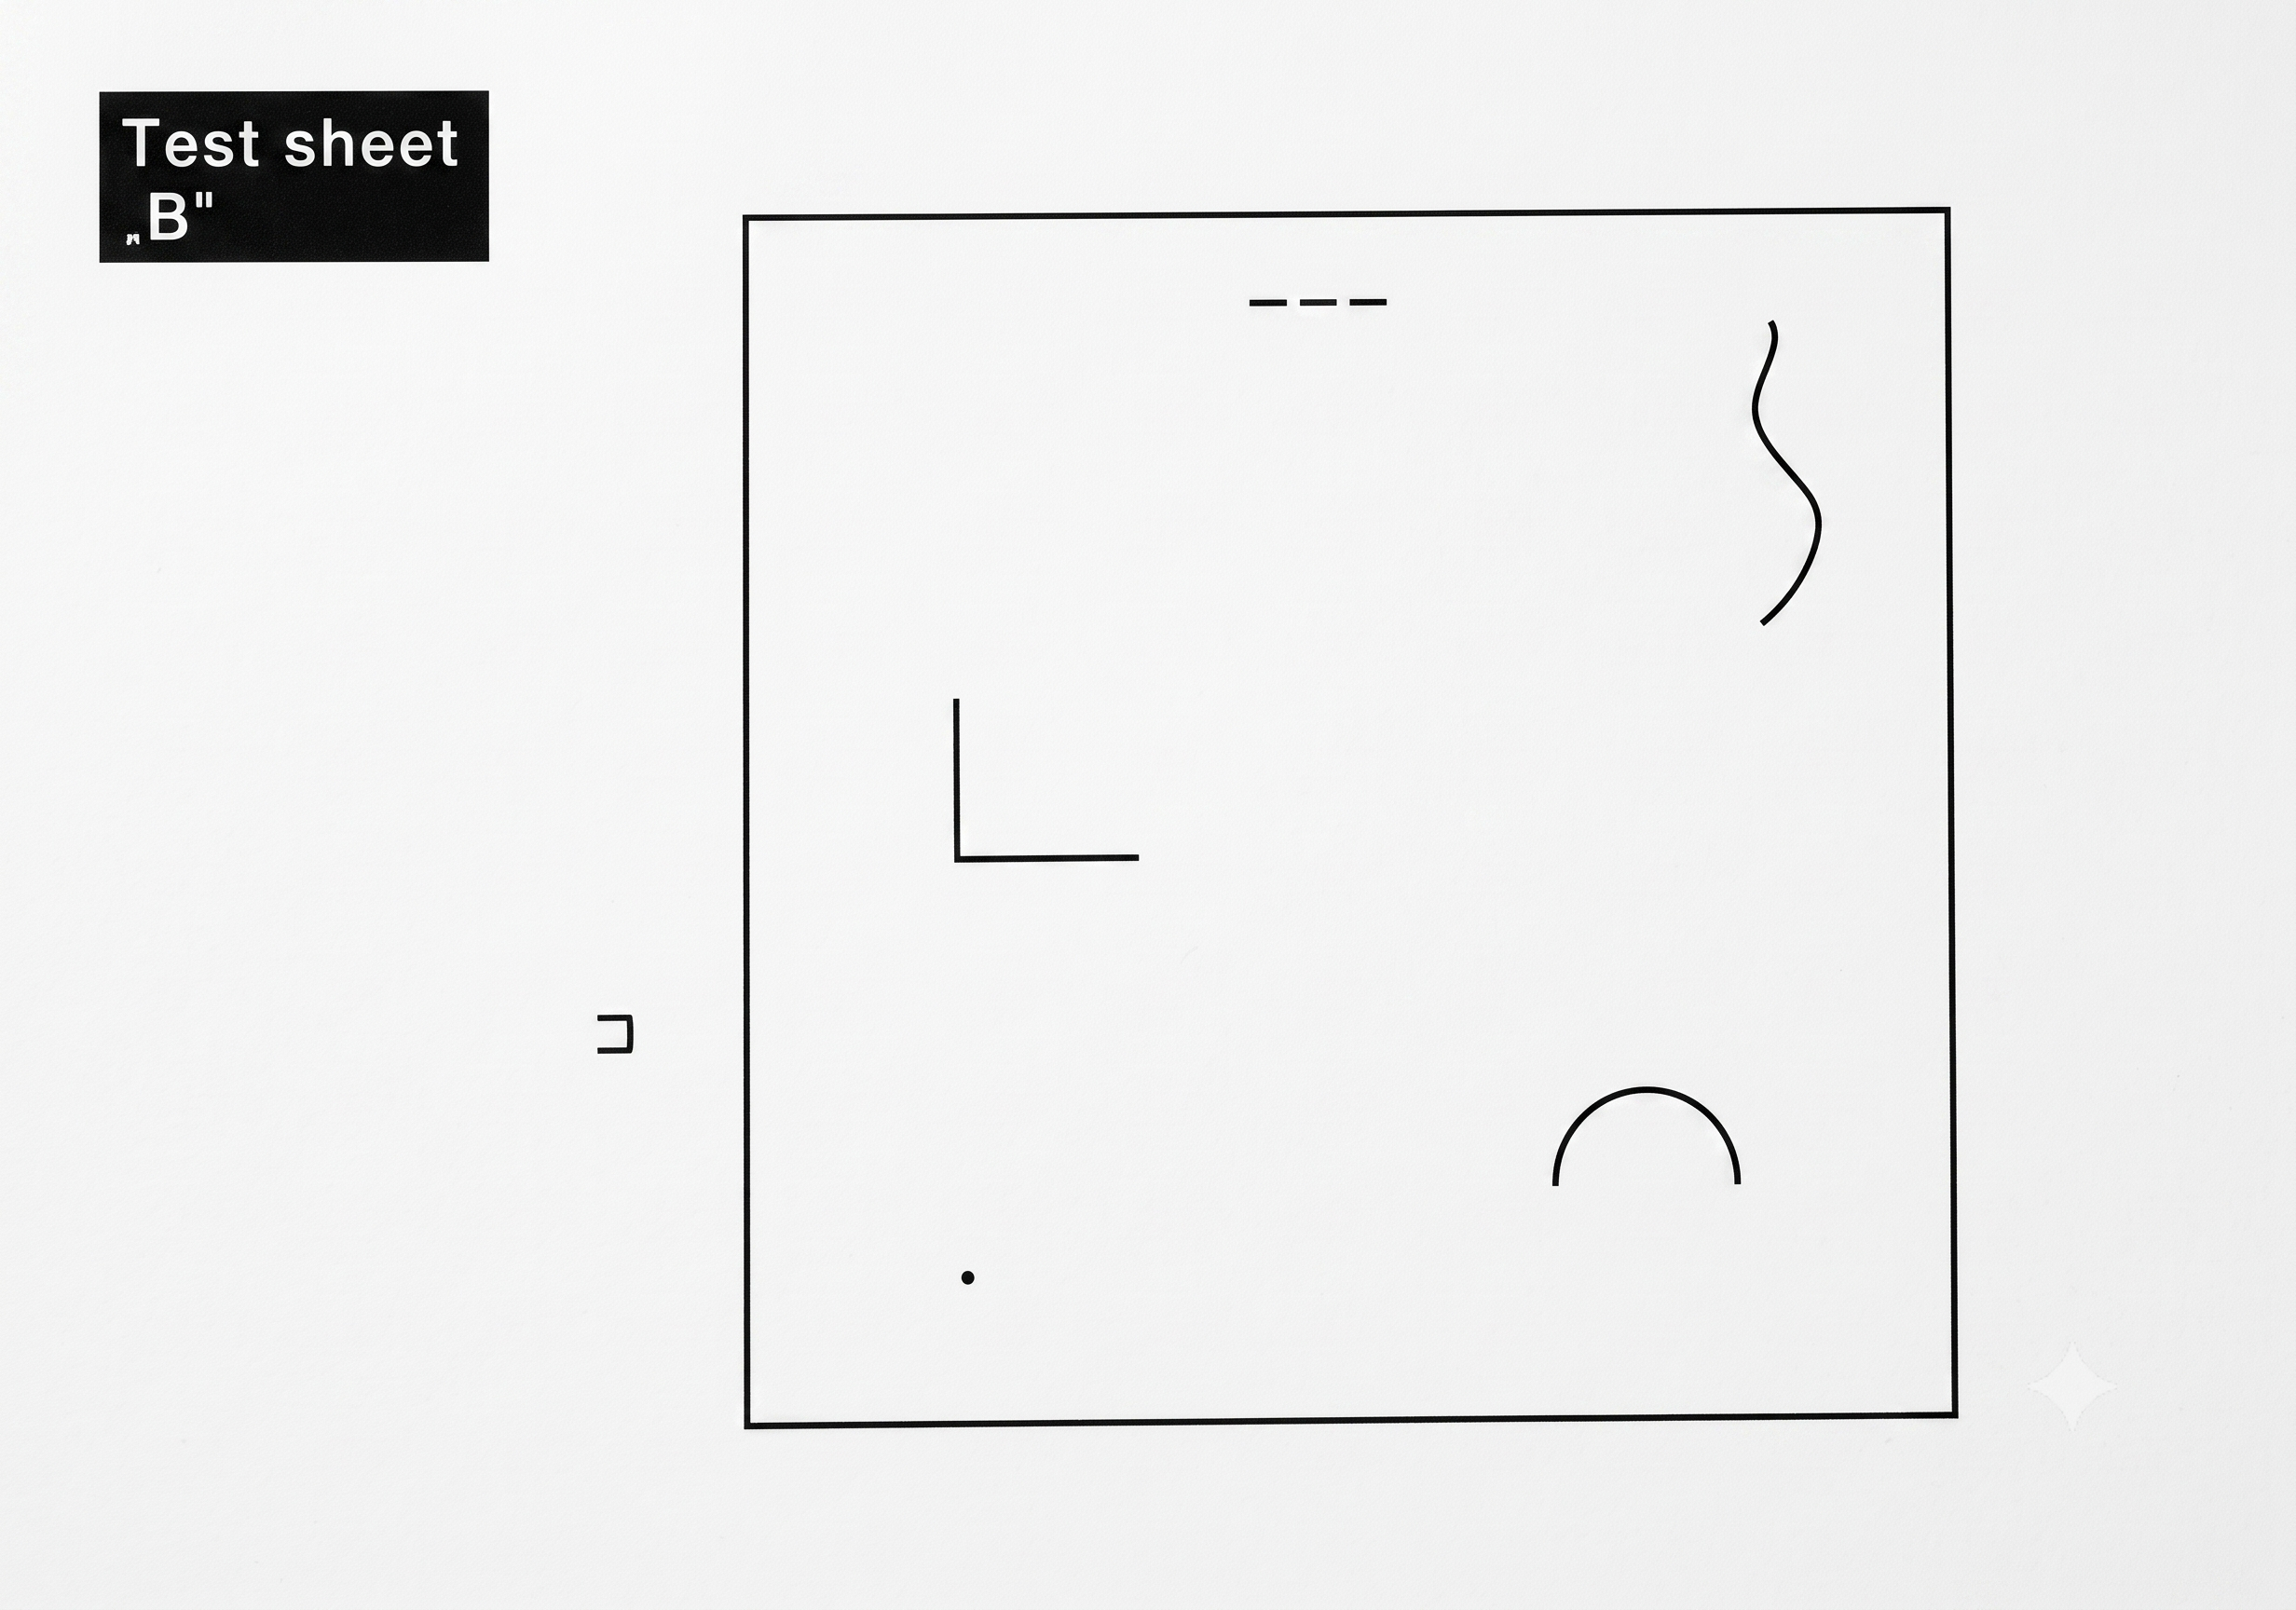
\includegraphics[width=\textwidth]{figures/test_sheet_B.png}
        \caption{Version B}
        \label{fig:test_sheet_b}
    \end{subfigure}
    \caption{Les deux versions de la feuille TCT-DP, selon le sens d'impression.}
    \label{fig:test_sheet}
\end{figure}

La population ciblée pour la passation principale d'octobre/novembre 2026 est constituée d'étudiants.

% Les trois conditions expérimentales :
\subsubsection{Condition C0 : feedback neutre (groupe contrôle)}

En condition C0, le robot délivre à chaque tour un feedback neutre et générique, sans faire référence au contenu précis du dessin ni orienter le participant (figure~\ref{fig:c0_example}). Cette condition sert de groupe contrôle : elle isole l'effet de la simple présence attentive du robot, sans apport créatif de sa part. La phrase est tirée aléatoirement dans une banque de dix formulations par tour (reproduite en annexe~\ref{annexe:feedback_c0}).

\begin{figure}[H]
    \centering
    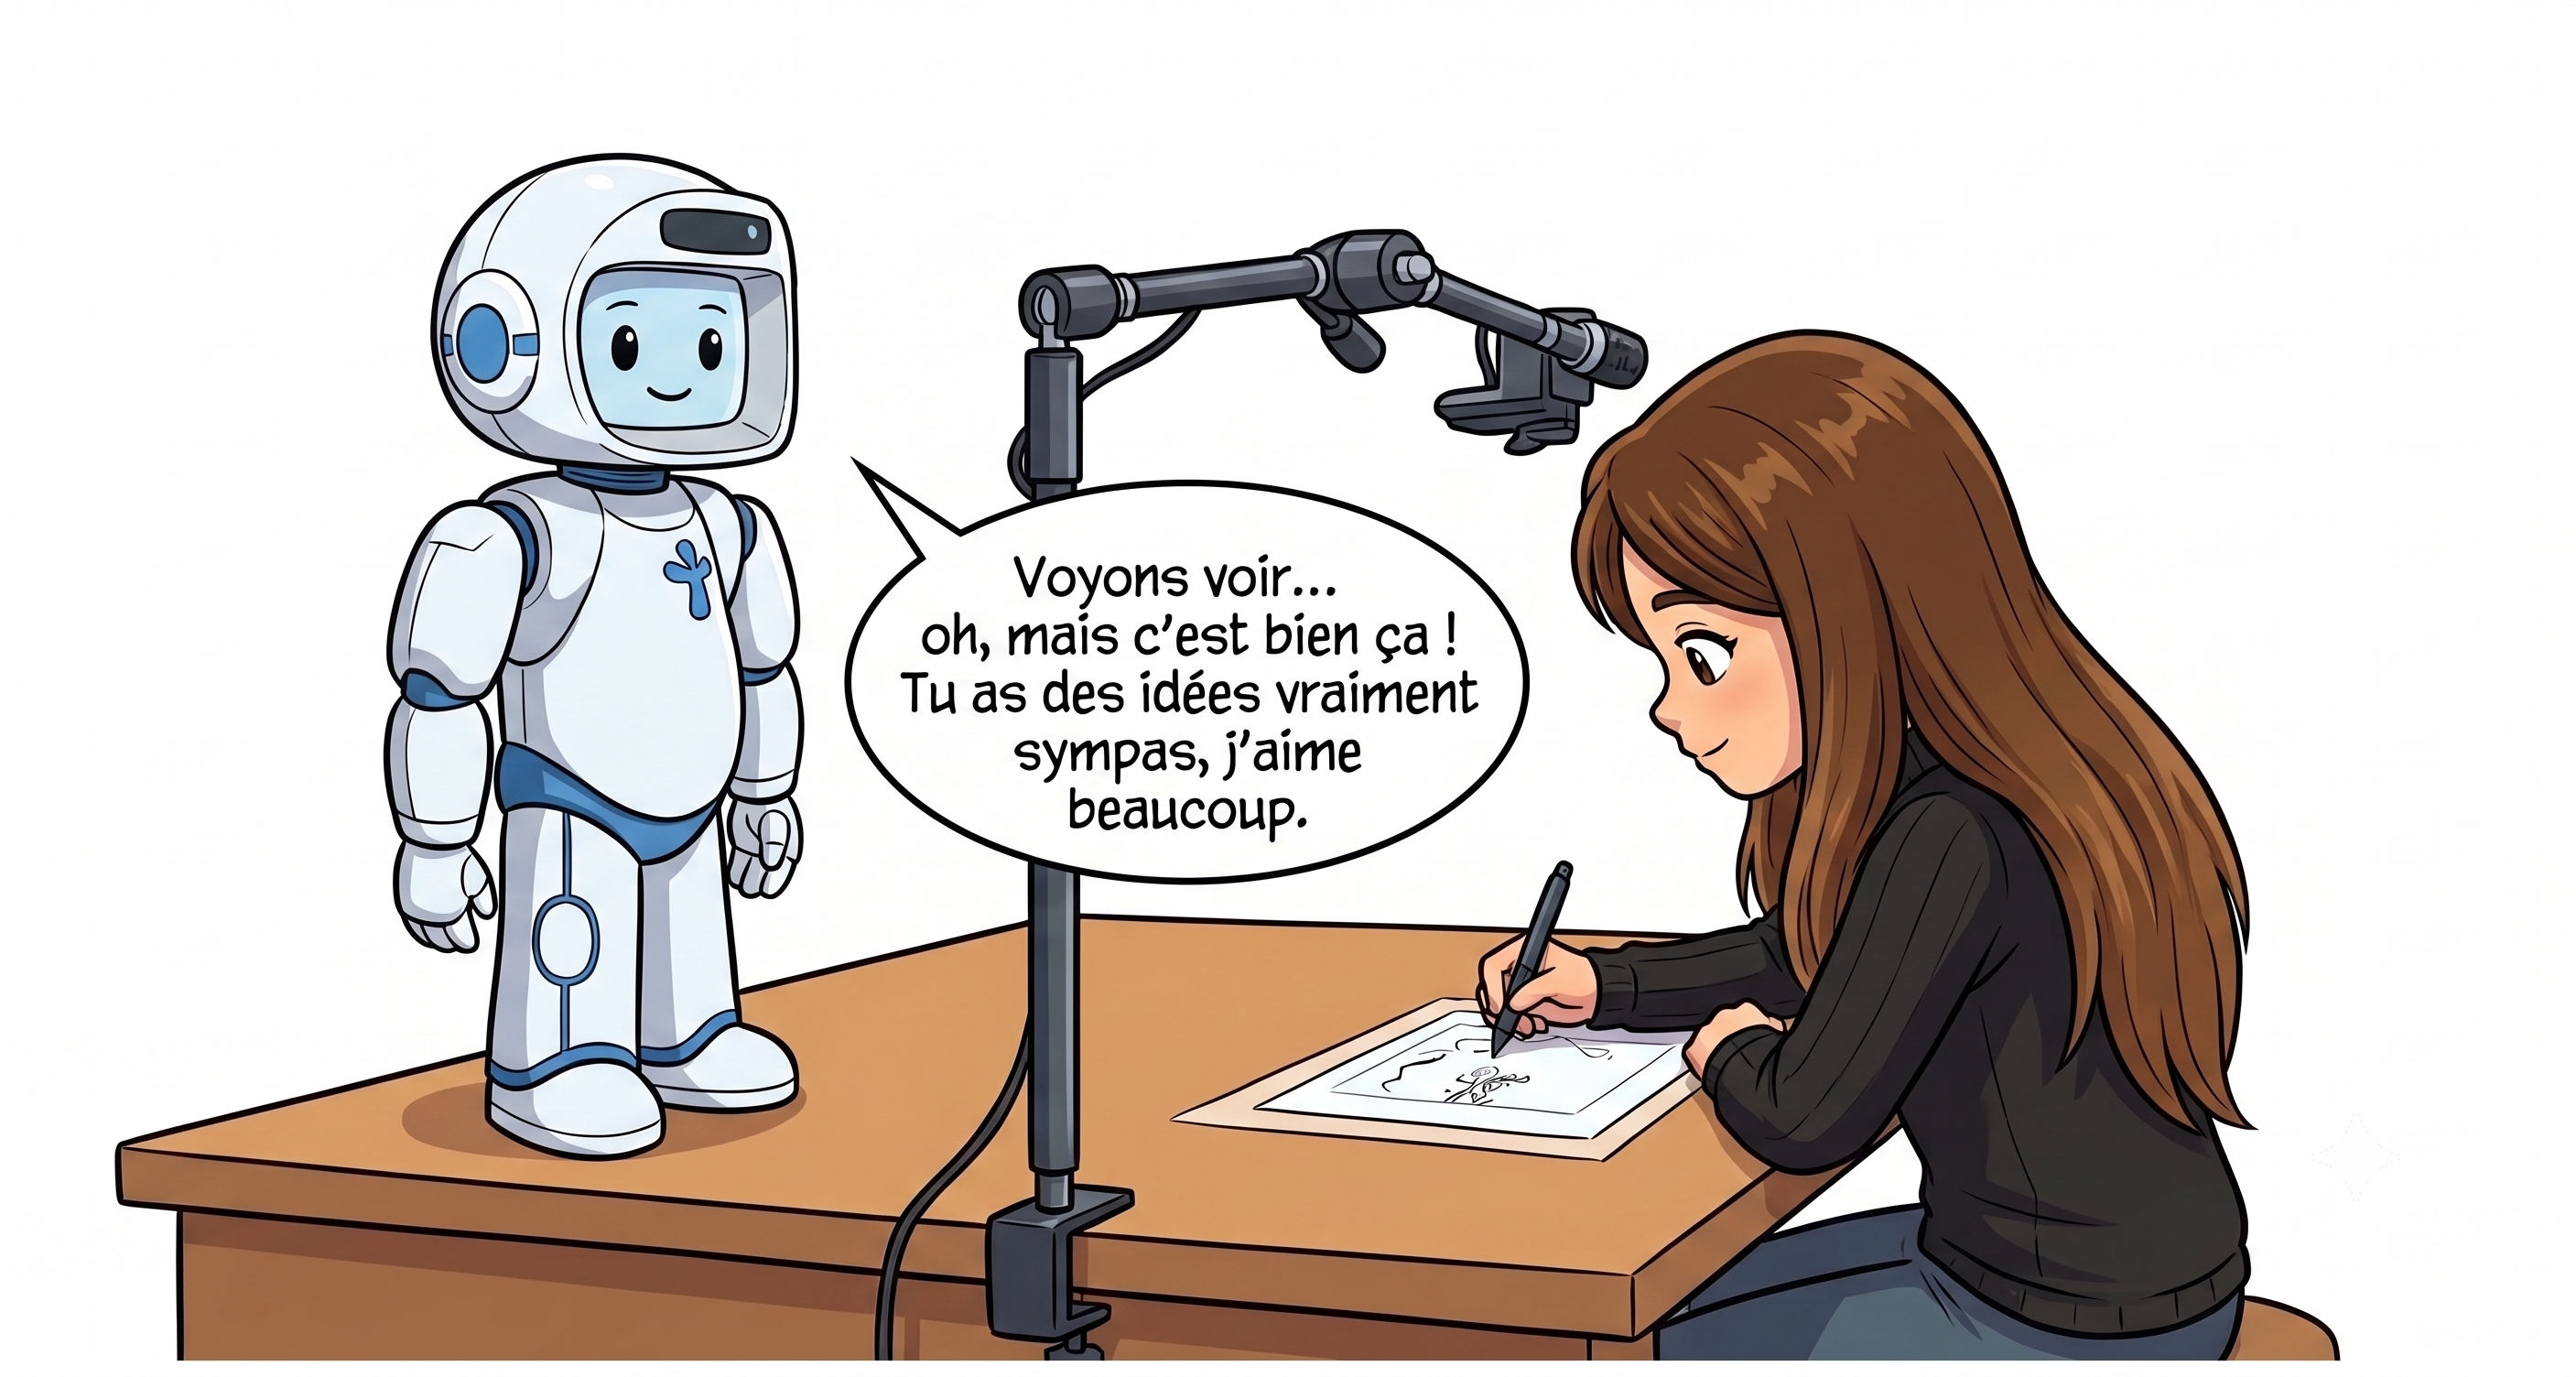
\includegraphics[width=0.85\textwidth]{figures/feedback_C0.png}
    \caption{Exemple de feedback en condition C0.}
    \label{fig:c0_example}
\end{figure}

\subsubsection{Condition C1 : échange piloté par un modèle de langage}
\label{sec:condition_c1}

En condition C1, le robot engage un échange piloté par un modèle de langage, mêlant questions et suggestions légères portant sur le dessin du participant (figure~\ref{fig:c1_example}). Concrètement, une photo de sa feuille est prise à la fin du tour, puis analysée par un modèle vision-langage pour en tirer une description du dessin ; cette description alimente ensuite le modèle de langage, qui s'appuie dessus pour formuler ses interventions de façon contextualisée plutôt que générique. L'échange suit toujours la même logique en trois temps : au premier tour, le robot pose systématiquement une question ; au deuxième tour, il relance sous la forme d'une suggestion formulée elle-même comme une question ; au troisième tour, il propose une suggestion légère. Le prompt complet est reproduit en annexe~\ref{annexe:prompt_c1}.

\begin{figure}[H]
    \centering
    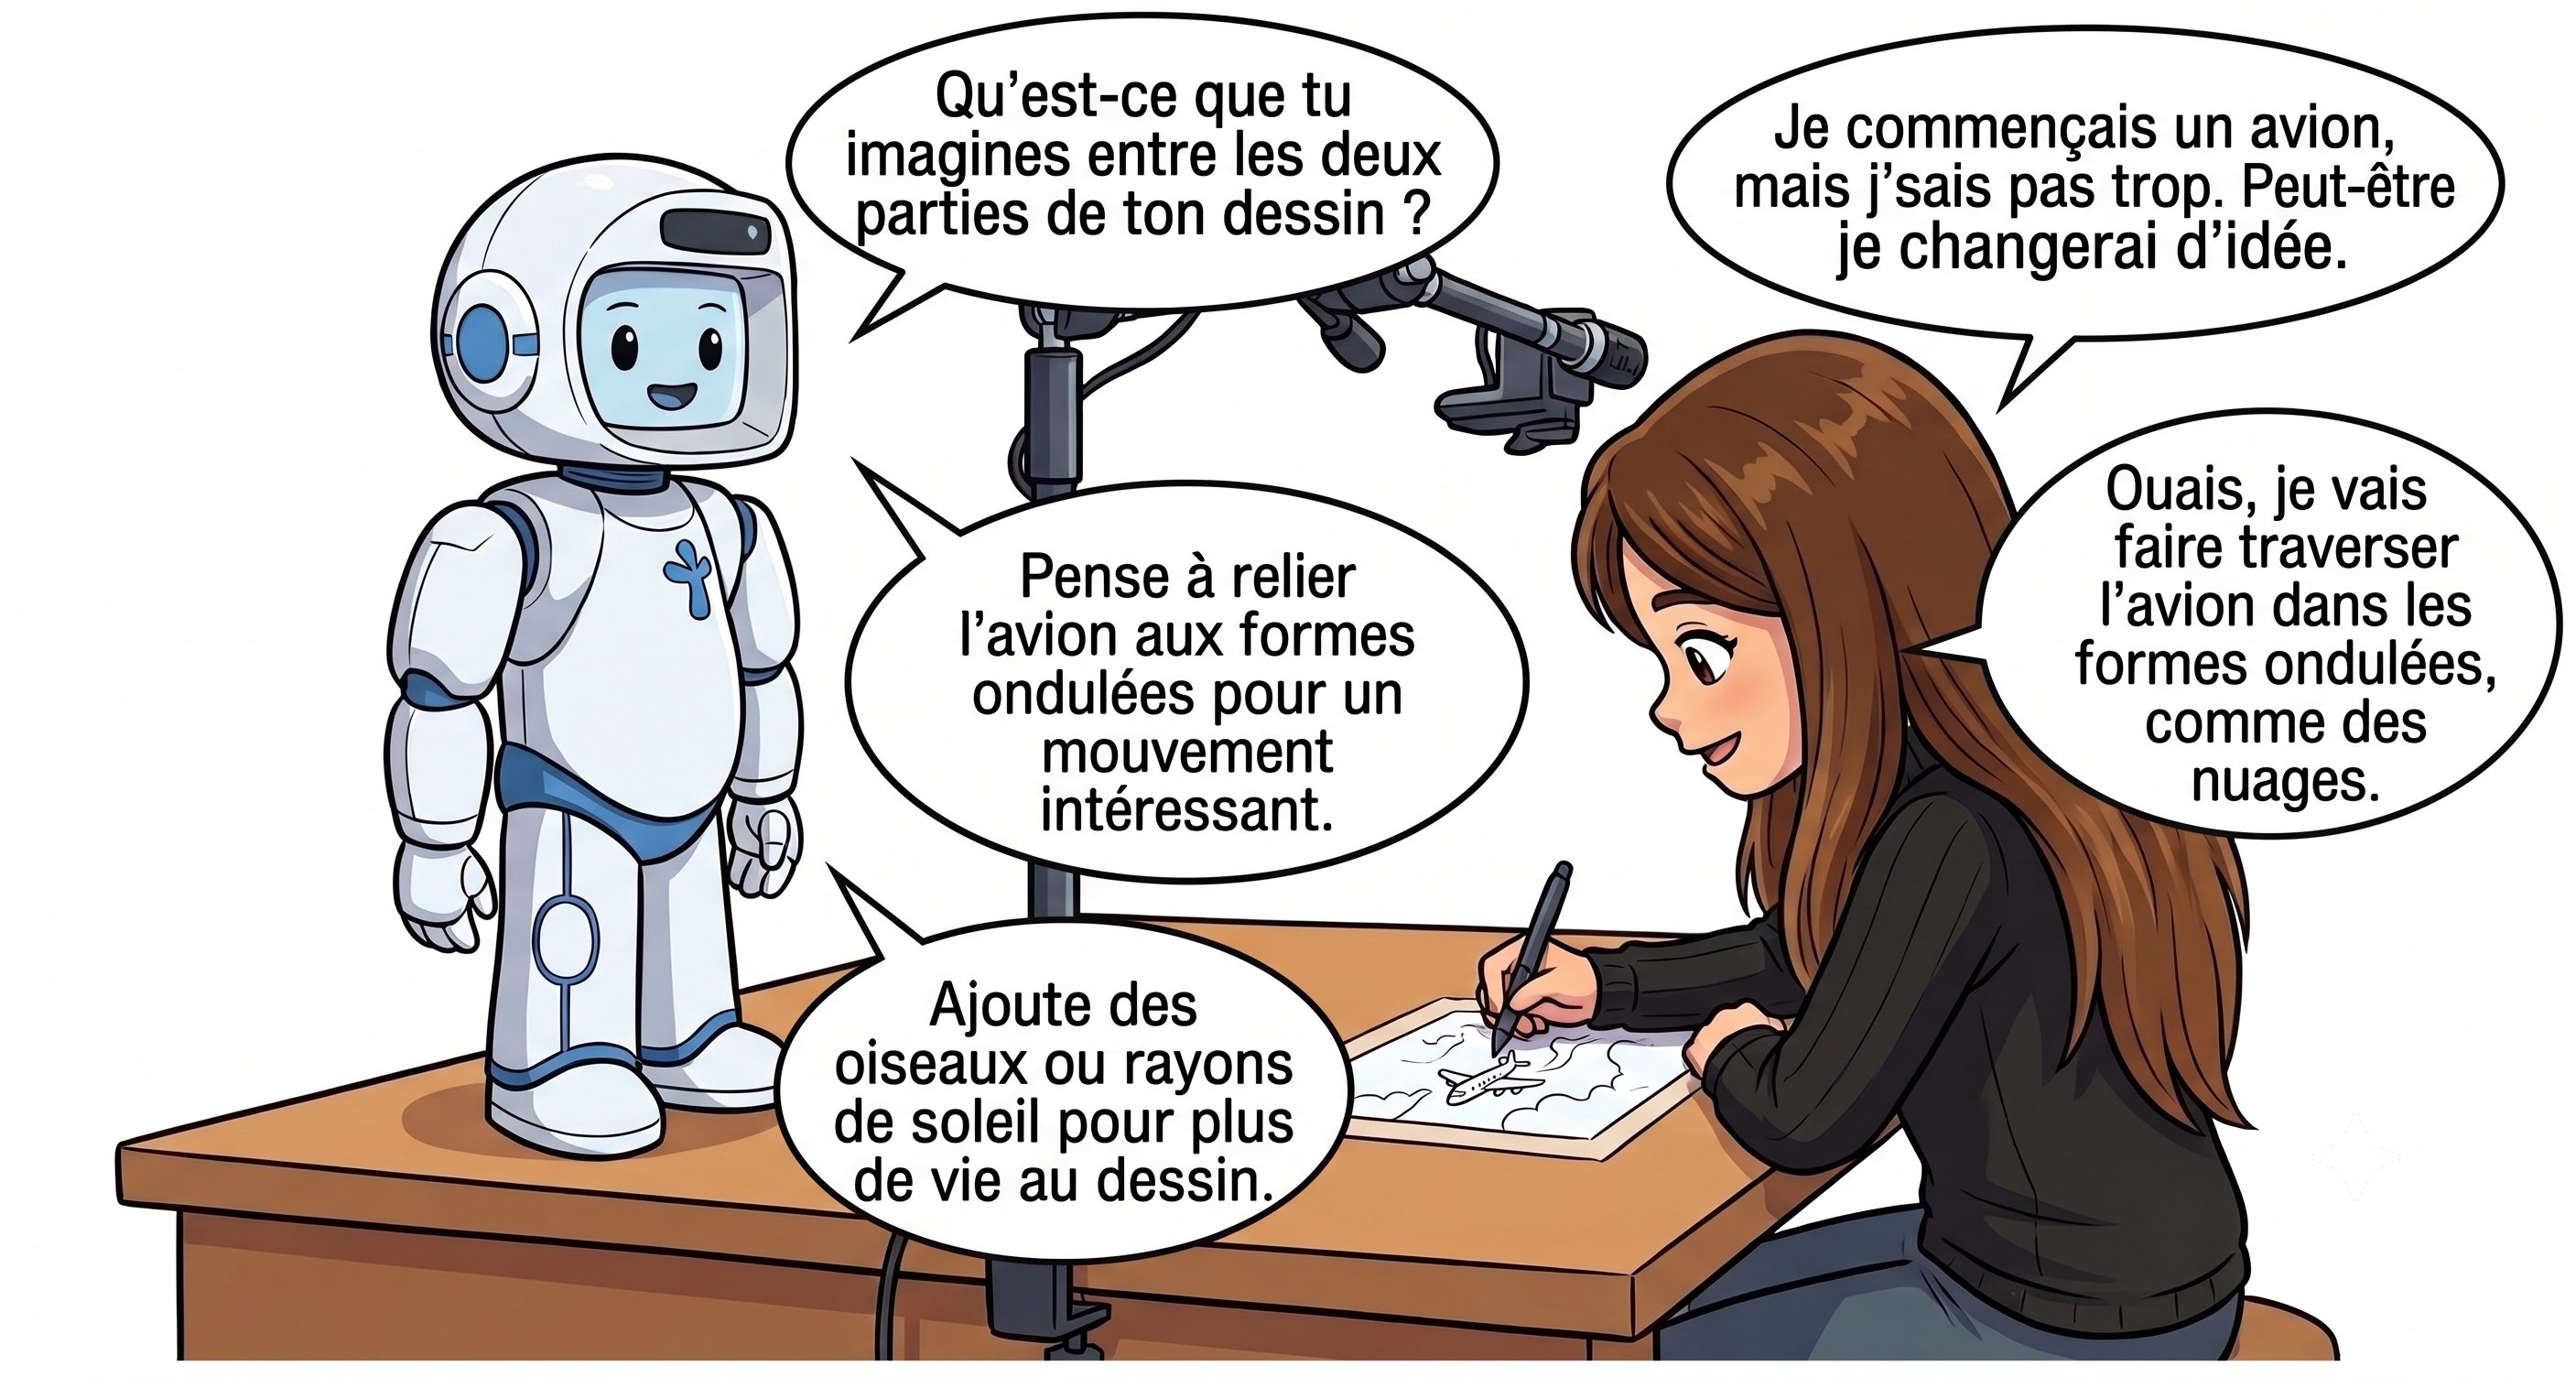
\includegraphics[width=0.85\textwidth]{figures/feedback_C1.png}
    \caption{Exemple illustratif d'échange en condition C1.}
    \label{fig:c1_example}
\end{figure}

\subsubsection{Condition C2 : feedback visuel génératif (projection)}

En condition C2, le robot invite le participant à regarder une proposition visuelle de son dessin, générée puis projetée sur un mur (figure~\ref{fig:c2_example}). Concrètement, le système génère une image en se basant sur ce que le participant a lui-même dessiné : une photo de sa feuille est prise à la fin du tour, puis un modèle génératif produit une version augmentée du dessin, qui complète les éléments du test TCT-DP non encore utilisés et ajoute également de nouveaux éléments s'intégrant au dessin existant, tout en respectant le style et les traits déjà posés par le participant. Cette proposition est ensuite montrée au participant à l'aide d'un vidéoprojecteur qui l'affiche sur un mur de la pièce, et le robot prononce une courte phrase qui l'invite à regarder cette proposition et à en faire ce qu'il veut, qu'il choisisse de s'en inspirer ou de continuer selon sa propre vision. Le prompt complet est reproduit en annexe~\ref{annexe:prompt_c2}.

\begin{figure}[H]
    \centering
    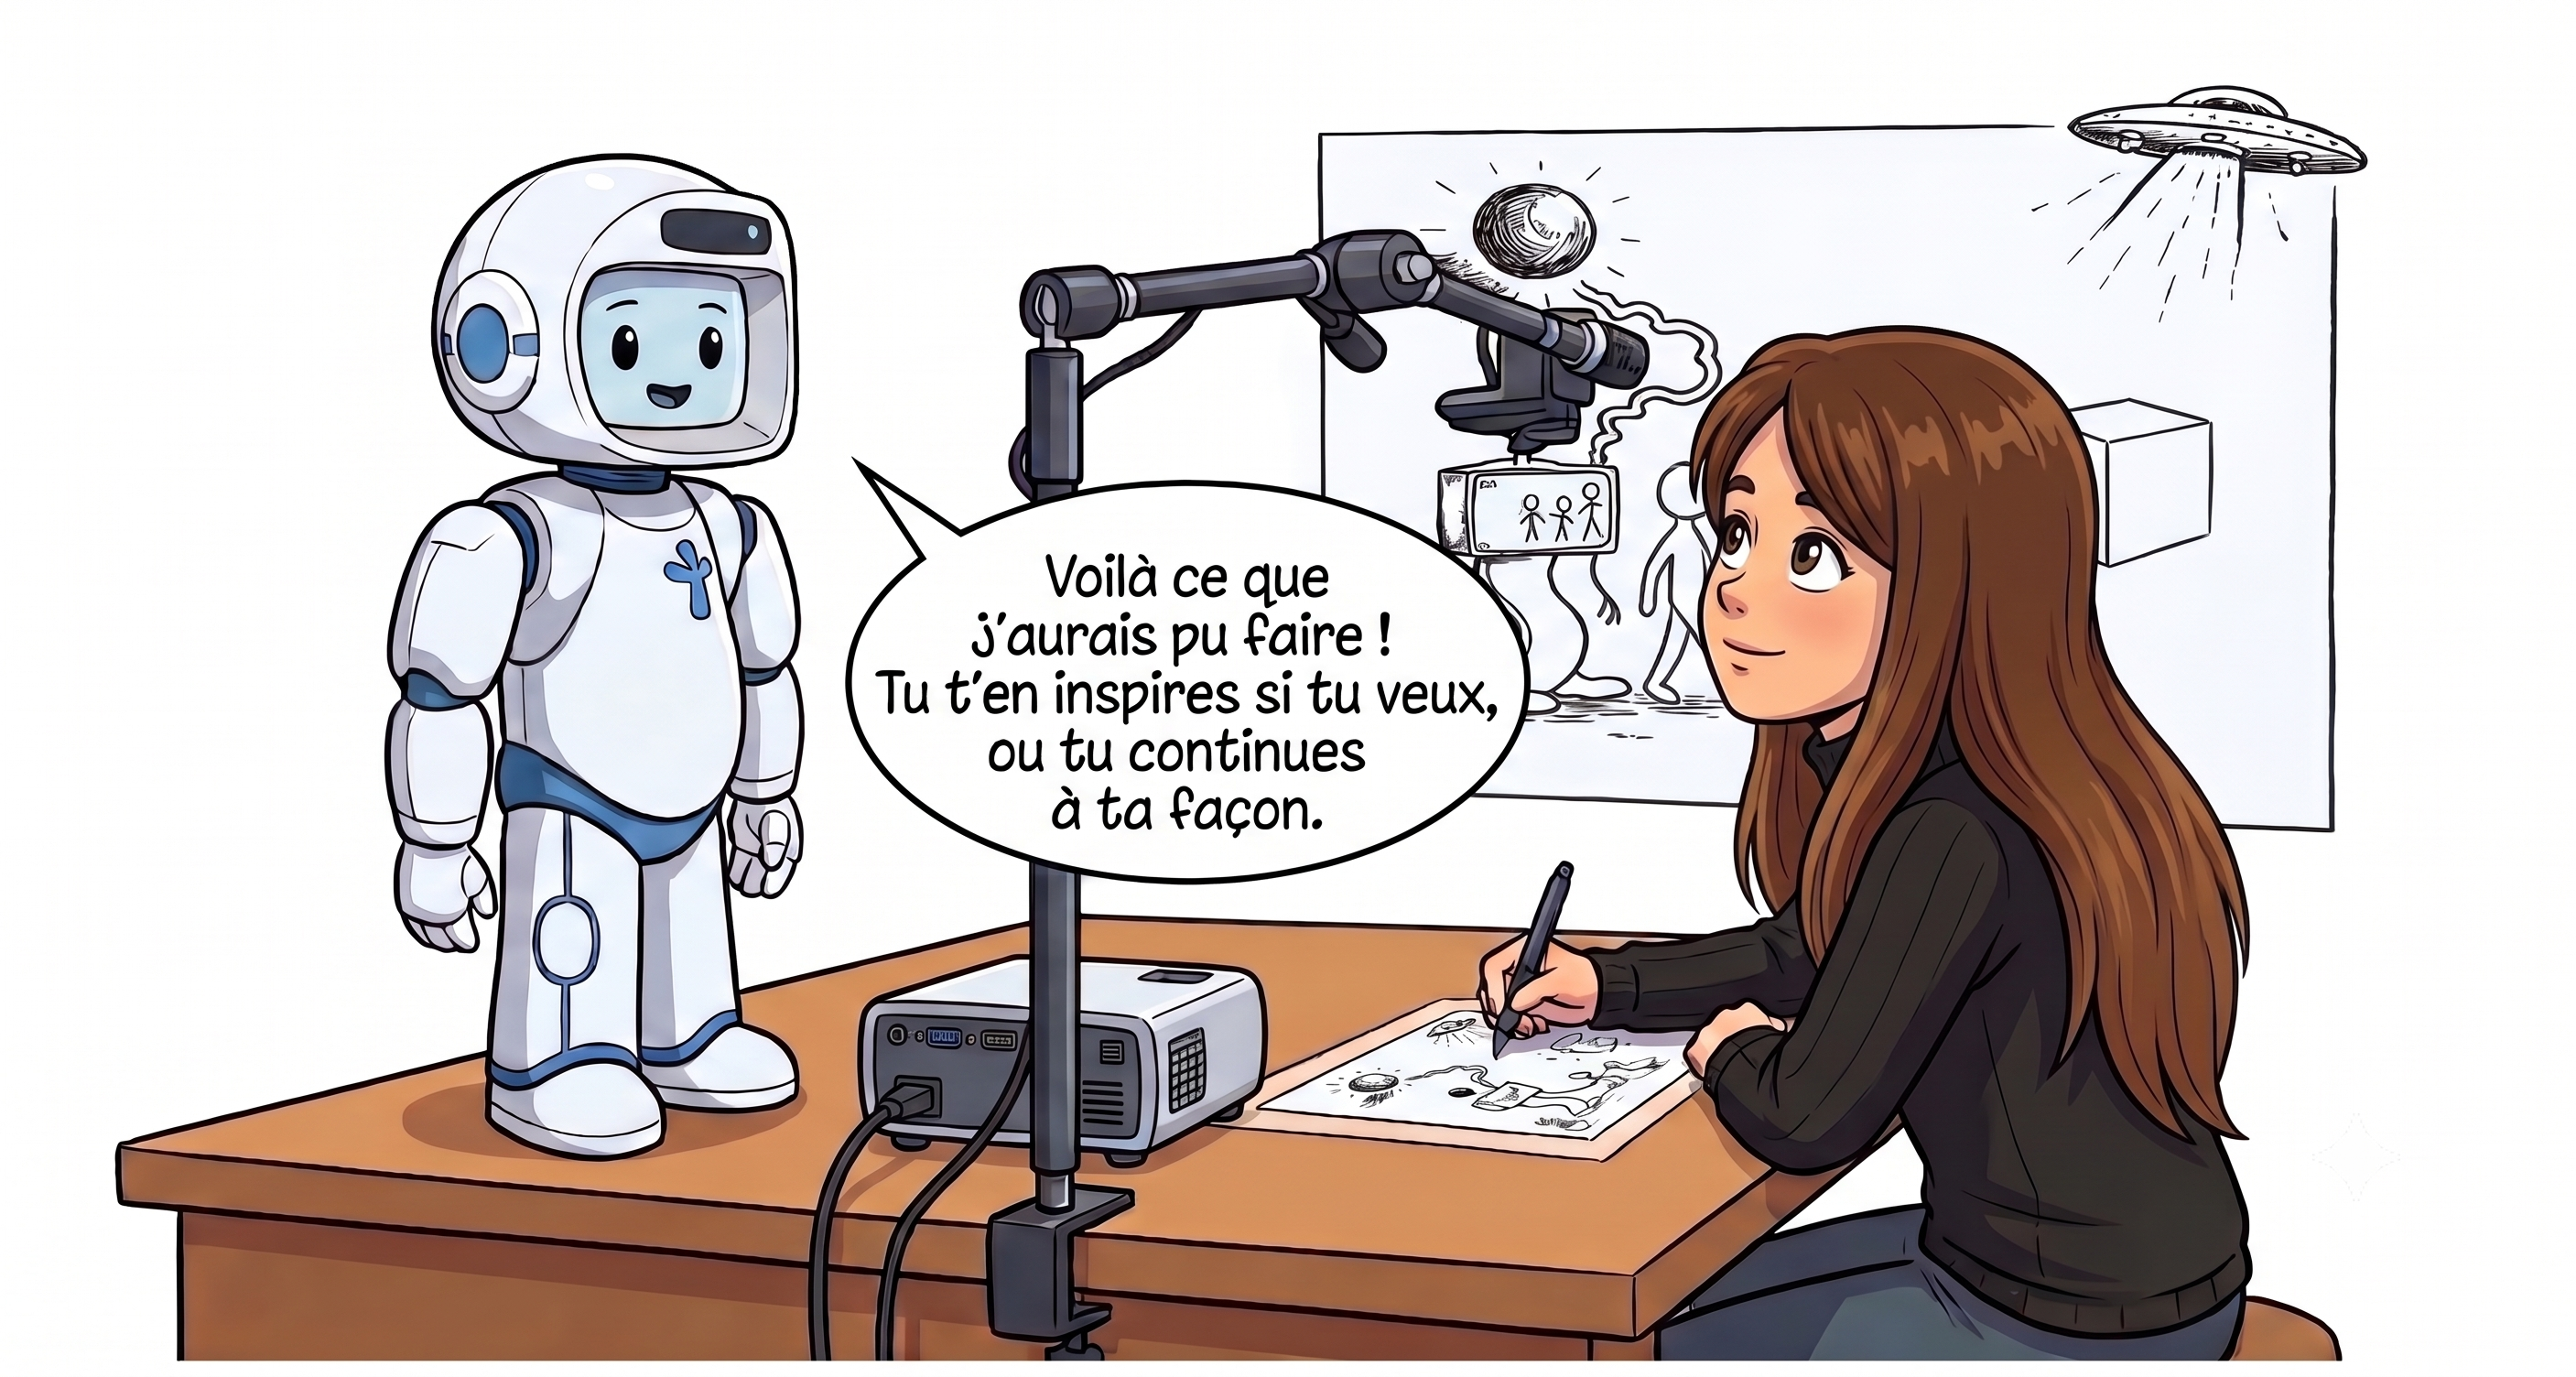
\includegraphics[width=0.85\textwidth]{figures/feeedback_C2.png}
    \caption{Exemple de dessin projeté en condition C2.}
    \label{fig:c2_example}
\end{figure}

\subsubsection{Les sept phases de l'expérience}

L'expérience se déroule en sept phases successives, illustrées en figure~\ref{fig:session}. Elle débute par une phase d'introduction (\texttt{INTRO}), pendant laquelle le robot se présente au participant et attend une confirmation orale de sa part pour démarrer. Suit une phase de ice breaking (\texttt{ICE\_BREAKING}), un court échange de trois interventions amicales visant à mettre le participant à l'aise avant la tâche. La troisième phase (\texttt{TASK\_INTRO}) consiste en l'explication par le robot des consignes du test TCT-DP.

Vient ensuite la phase de dessin (\texttt{DRAWING}), durant laquelle le participant dispose de 90 secondes pour dessiner, suivie d'une phase de feedback (\texttt{FEEDBACK}) durant laquelle le robot adresse un retour au participant selon la condition expérimentale décrite ci-dessus. Ce cycle dessin puis feedback est répété trois fois avant de passer à la suite. Enfin, l'expérience se referme sur deux dernières phases : le robot observe une dernière fois le dessin pour lui proposer un titre (\texttt{TITLE}), puis salue le participant et met fin à la session (\texttt{ENDING}).

\begin{figure}[H]
    \centering
    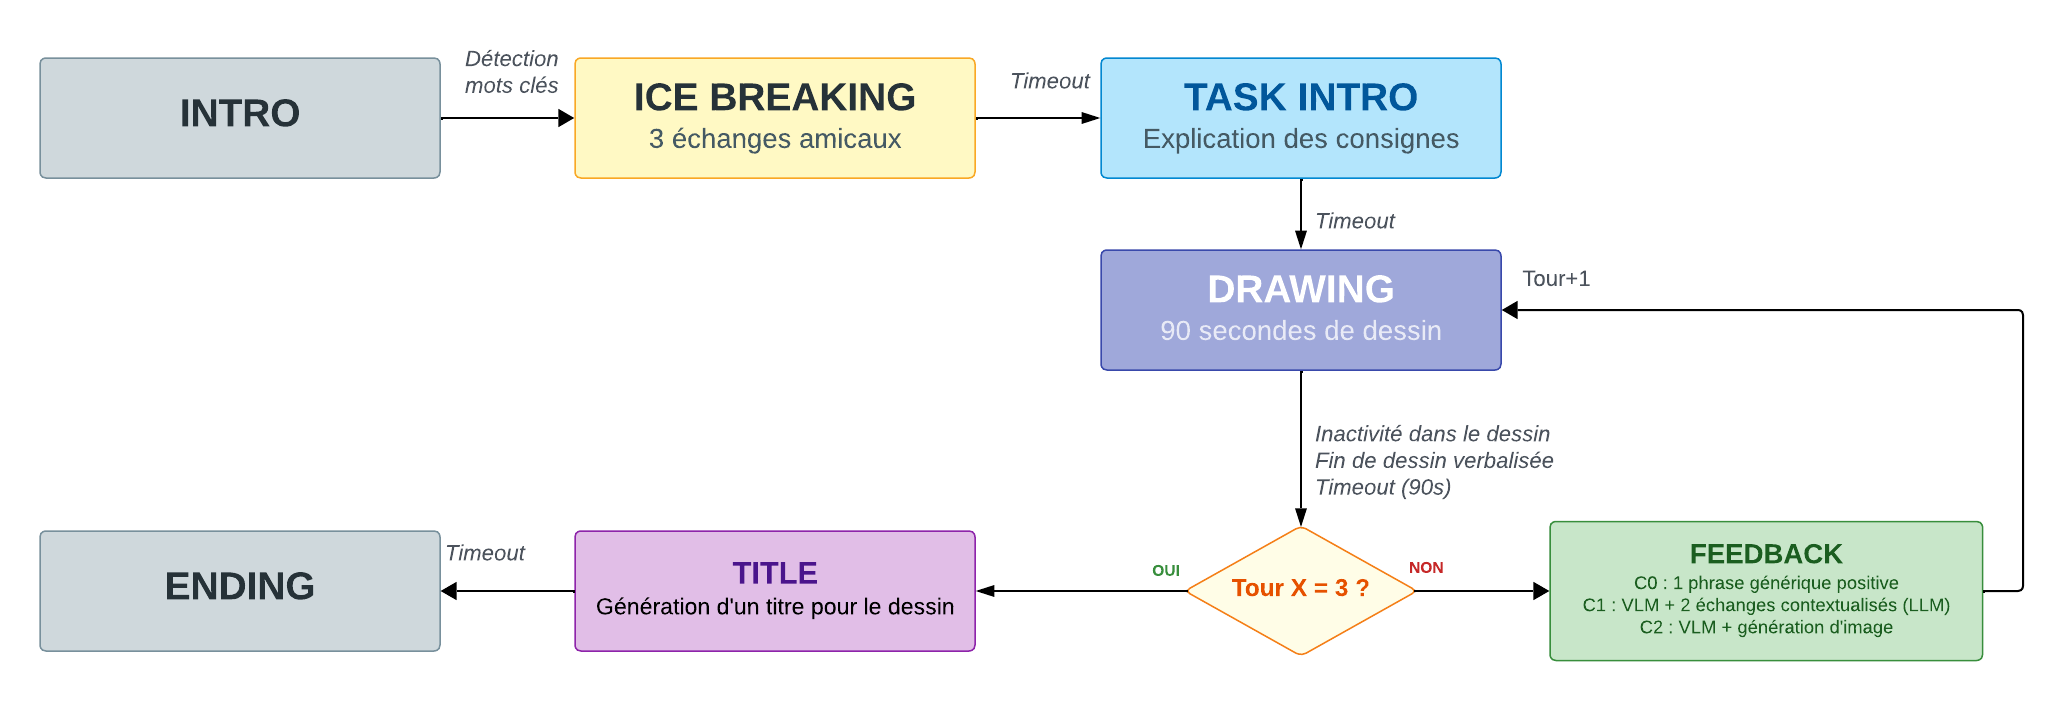
\includegraphics[width=\textwidth]{figures/session_crearobot.png}
    \caption{Déroulement d'une session CreaRobot et logique de transition entre les phases.}
    \label{fig:session}
\end{figure}

\subsubsection{Critères de scoring TCT-DP}

La cotation du TCT-DP repose sur une grille de critères propre au test, définie par ses auteurs pour évaluer la production graphique du participant \cite{urbanjellen1996,urban2005}. Le tableau~\ref{tab:tct_dp_criteres} liste l'ensemble de ces critères.

\begin{table}[H]
    \centering
    \begin{tabular}{@{}llp{6cm}c@{}}
        \toprule
        \textbf{Code} & \textbf{Critère} & \textbf{Description} & \textbf{Score max} \\
        \midrule
        Cn    & Continuations               & Utilisation ou extension des six fragments fournis & /6 \\
        Cm    & Complétions                 & Ajouts et compléments aux fragments utilisés & /6 \\
        Ne    & Nouveaux éléments           & Tout nouveau symbole ou figure ajouté & /6 \\
        Cl    & Connexions (ligne)          & Connexion entre fragments par une ligne & /6 \\
        Cth   & Connexions (thème)          & Composition thématique cohérente (gestalt) & /6 \\
        Bfd   & Bris de frontière (d)       & Utilisation du petit carré hors du cadre & /3 \\
        Bfi   & Bris de frontière (i)       & Tout débordement hors du cadre & /3 \\
        Pe    & Perspective                 & Rupture avec la 2D, effets 3D & /6 \\
        Hu    & Humour et affectivité       & Dessin humoristique ou à forte expressivité & /3 \\
        \rowcolor{gray!15} Uc-a & Inconventionnalité (a) & Manipulation du matériel de test (non utilisé, voir ci-dessous) & --- \\
        Uc-b  & Inconventionnalité (b)      & Élément surréaliste & /2 \\
        Uc-c  & Inconventionnalité (c)      & Utilisation de symboles & /2 \\
        Uc-d  & Inconventionnalité (d)      & Usage non conventionnel du matériel & /2 \\
        \rowcolor{gray!15} Sp   & Vitesse (critère optionnel) & Déduction selon le temps écoulé (non utilisé, voir ci-dessous) & --- \\
        \midrule
        \multicolumn{3}{r}{\textbf{Total}} & \textbf{/51} \\
        \bottomrule
    \end{tabular}
    \caption{Critères de cotation du TCT-DP. Les critères grisés ne sont pas utilisés dans ce protocole.}
    \label{tab:tct_dp_criteres}
\end{table}

Deux de ces critères, optionnels dans le test original, ne sont pas retenus dans ce protocole. Le critère Sp (vitesse) déduit des points en fonction du temps mis par le participant pour terminer, ce qui suppose une seule session de dessin en continu et à son propre rythme. Or dans CreaRobot, le dessin est découpé en trois tours de 90 secondes maximum chacun, entrecoupés de phases de feedback : même si un participant peut signaler oralement qu'il a fini avant la fin d'un tour, le temps total passé à dessiner ne reflète plus le même phénomène que dans le test original, puisqu'il est fragmenté par la structure de l'expérience plutôt que laissé à la seule initiative du participant. Le critère Uc-a (manipulation du matériel de test) n'est pas non plus utilisé : à la fin de chaque phase de dessin, la feuille doit rester visible sous la caméra fixée au-dessus du participant pour être photographiée, ce qui ne laisse pas la possibilité de manipuler physiquement le support (le tourner, le déplacer, etc.).

Le score de créativité d'un dessin correspond à la somme des scores obtenus sur l'ensemble des critères retenus, sur un total de 51 points (tableau~\ref{tab:tct_dp_criteres}).

\newpage

\subsection{Architecture technique du système}

\subsubsection{Le robot QTRobot}
\label{sec:qtrobot}

\paragraph{Architecture matérielle et logicielle}

Le robot utilisé dans ce projet est un QTRobot V2 de la société LuxAI. Il s'agit d'un robot humanoïde de taille réduite, initialement conçu pour l'interaction sociale avec des enfants, notamment dans des contextes thérapeutiques auprès de personnes autistes (voir figure~\ref{fig:qtrobot}).

Le QTRobot repose sur deux unités de calcul embarquées reliées entre elles par câble Ethernet : une Raspberry Pi logée dans la tête (QTRP), qui initialise l'environnement ROS au démarrage, et un mini-PC situé dans le corps (QTPC). Les deux machines partagent le même espace ROS.

La figure~\ref{fig:archi_robot} présente l'ensemble des composants du robot. La répartition des périphériques suit une logique fonctionnelle : l'écran, les haut-parleurs, le réseau de microphones directionnels et les moteurs des bras sont rattachés au QTRP, tandis que la caméra 3D RealSense est connectée directement au QTPC. Deux ports sont également accessibles à l'arrière du robot : un port USB standard côté QTRP, et un port USB-C côté QTPC, permettant de brancher clavier, souris et écran via un hub.

\begin{figure}[H]
    \centering
    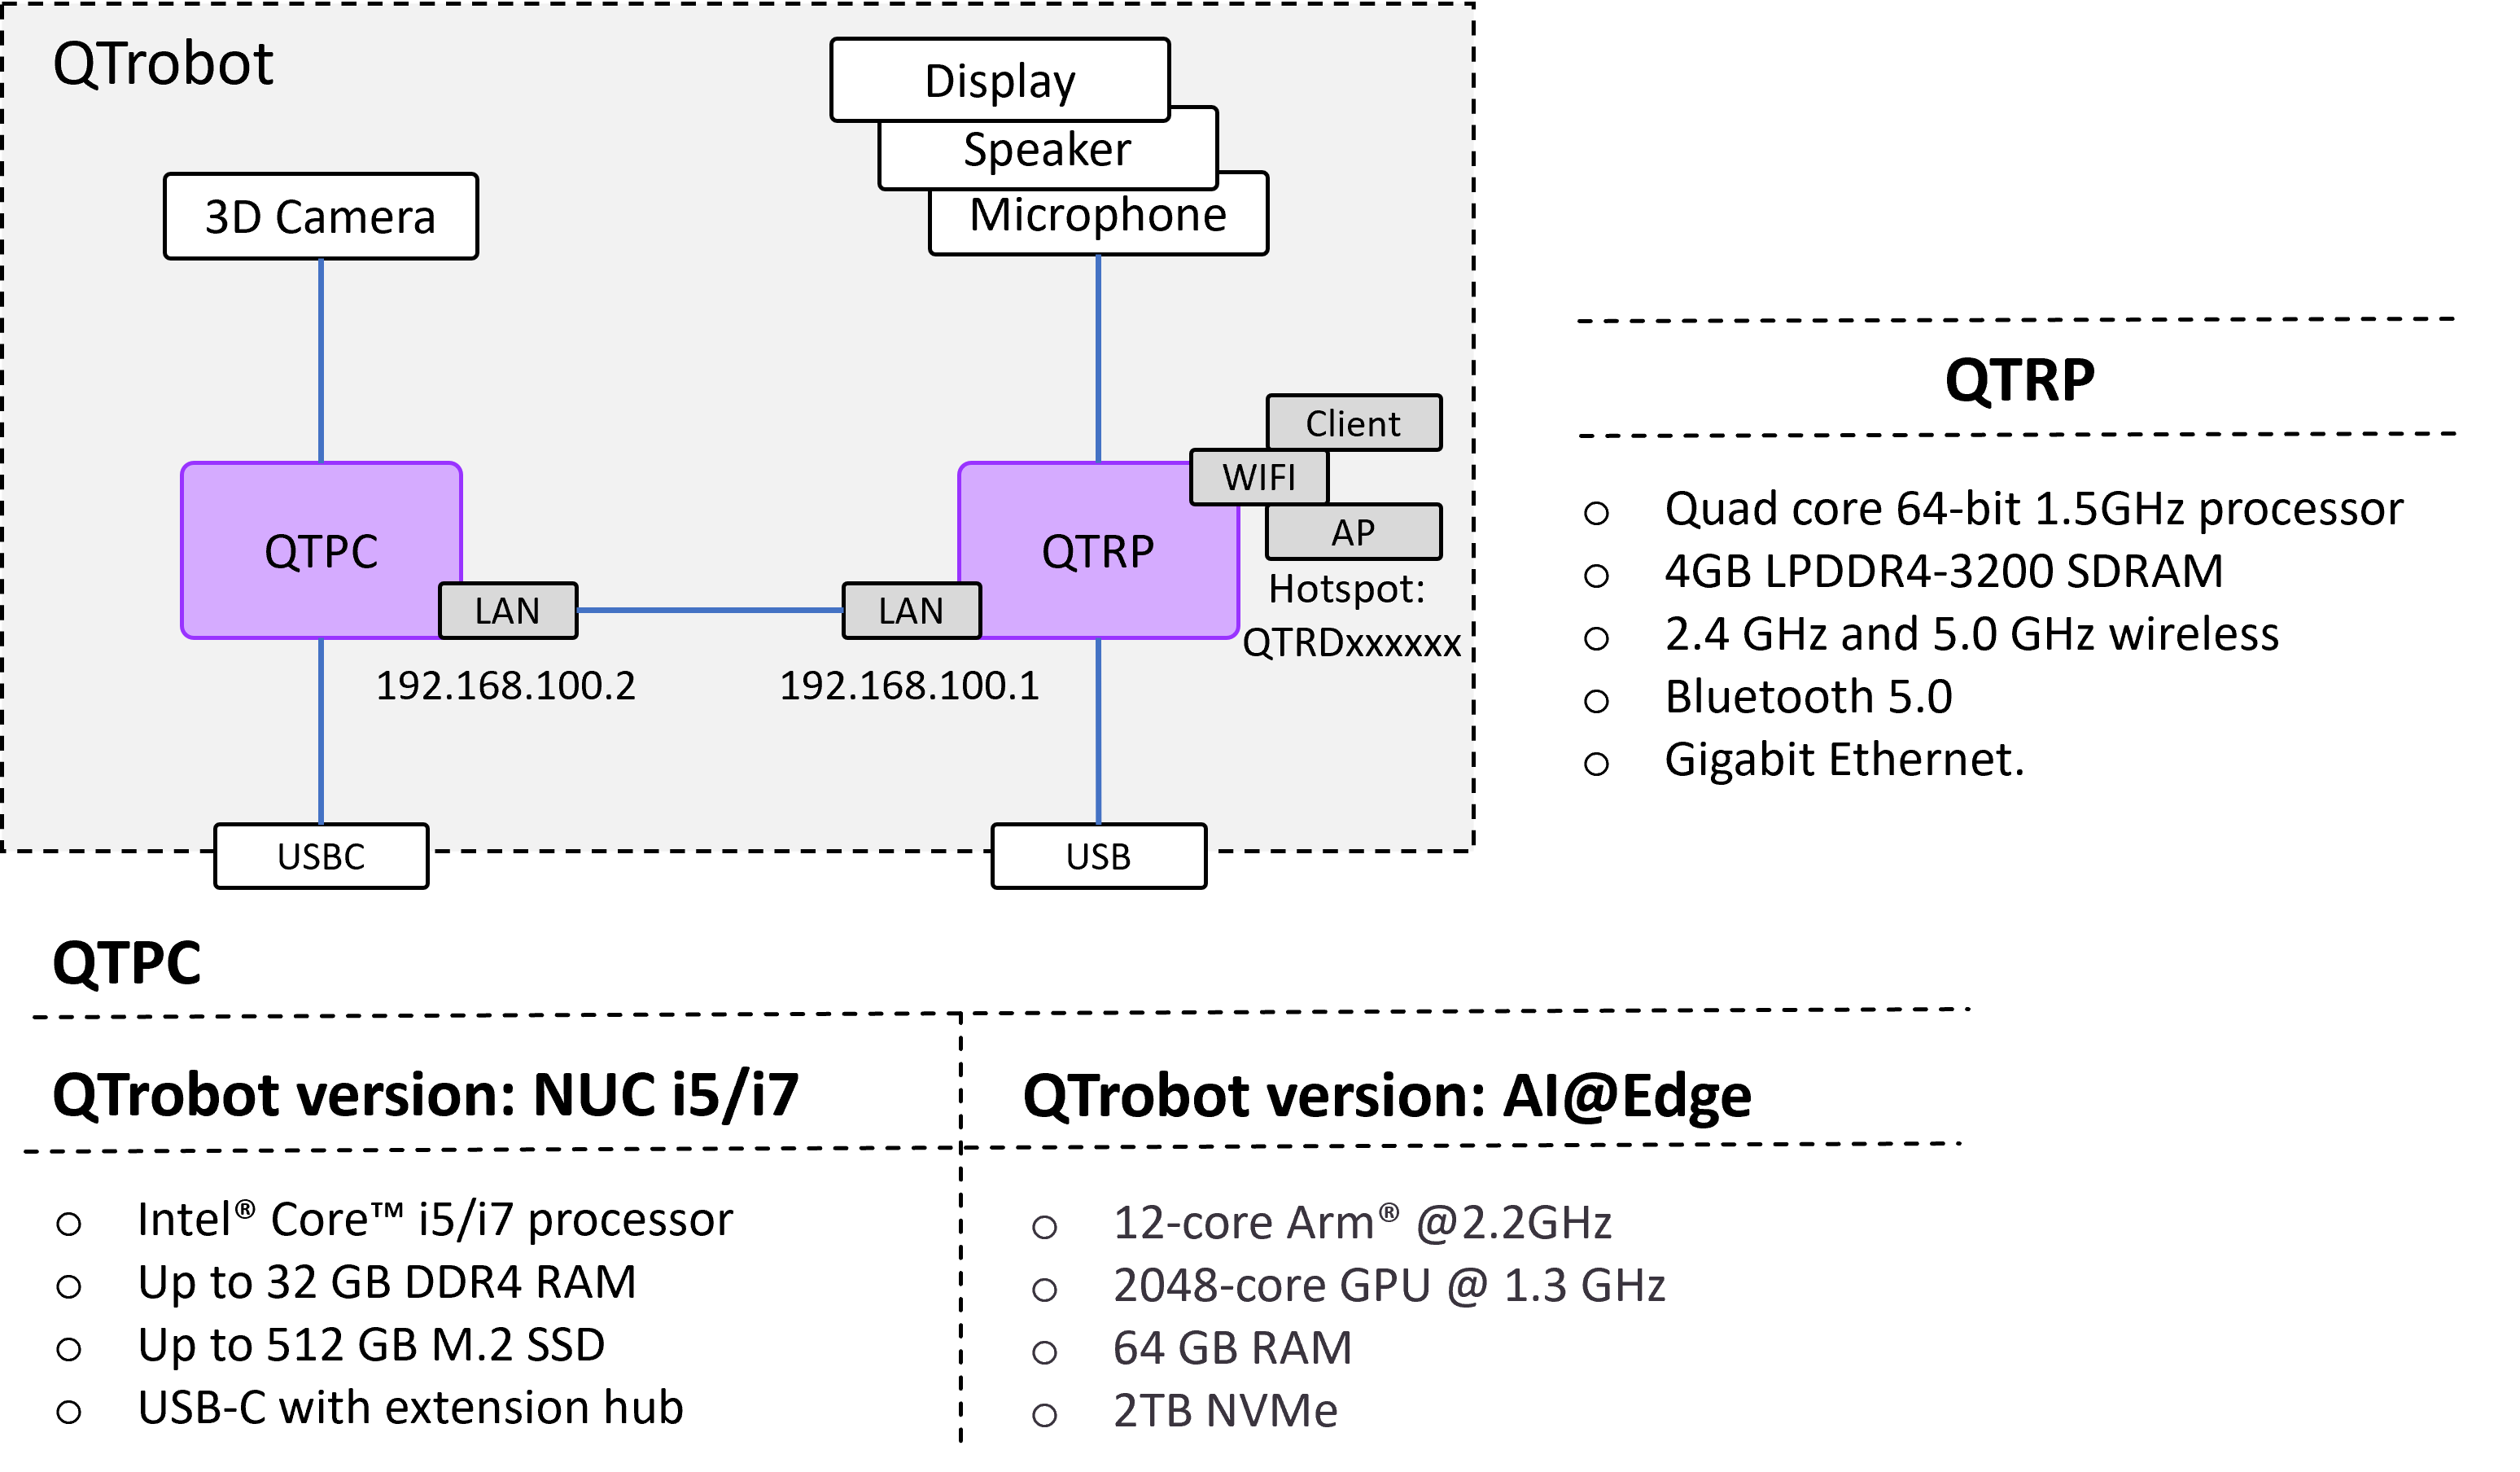
\includegraphics[width=0.75\textwidth]{figures/architecture_robot.png}
    \caption{Composants matériels du QTRobot V2~\cite{luxai_doc}.}
    \label{fig:archi_robot}
\end{figure}

Côté réseau, le QTPC dispose lui aussi d'une carte Wi-Fi, mais celle-ci est désactivée par LuxAI ; seule celle du QTRP est fonctionnelle, et elle ne peut assurer qu'un seul rôle à la fois : soit un point d'accès (\texttt{qt\_wlan0\_ap}), soit une connexion cliente vers un routeur existant (\texttt{qt\_wlan0\_client}) ; ces deux services sont mutuellement exclusifs et ne peuvent pas être actifs simultanément. Pour CreaRobot, le QTRP est configuré en mode client sur le réseau du LUTIN, à l'adresse \texttt{192.168.24.118} ; cette configuration est illustrée en figure~\ref{fig:archi_robot_network}, où le QTRP se connecte au routeur du réseau puis partage cette connexion internet vers le QTPC via leur lien Ethernet interne.

\begin{figure}[H]
    \centering
    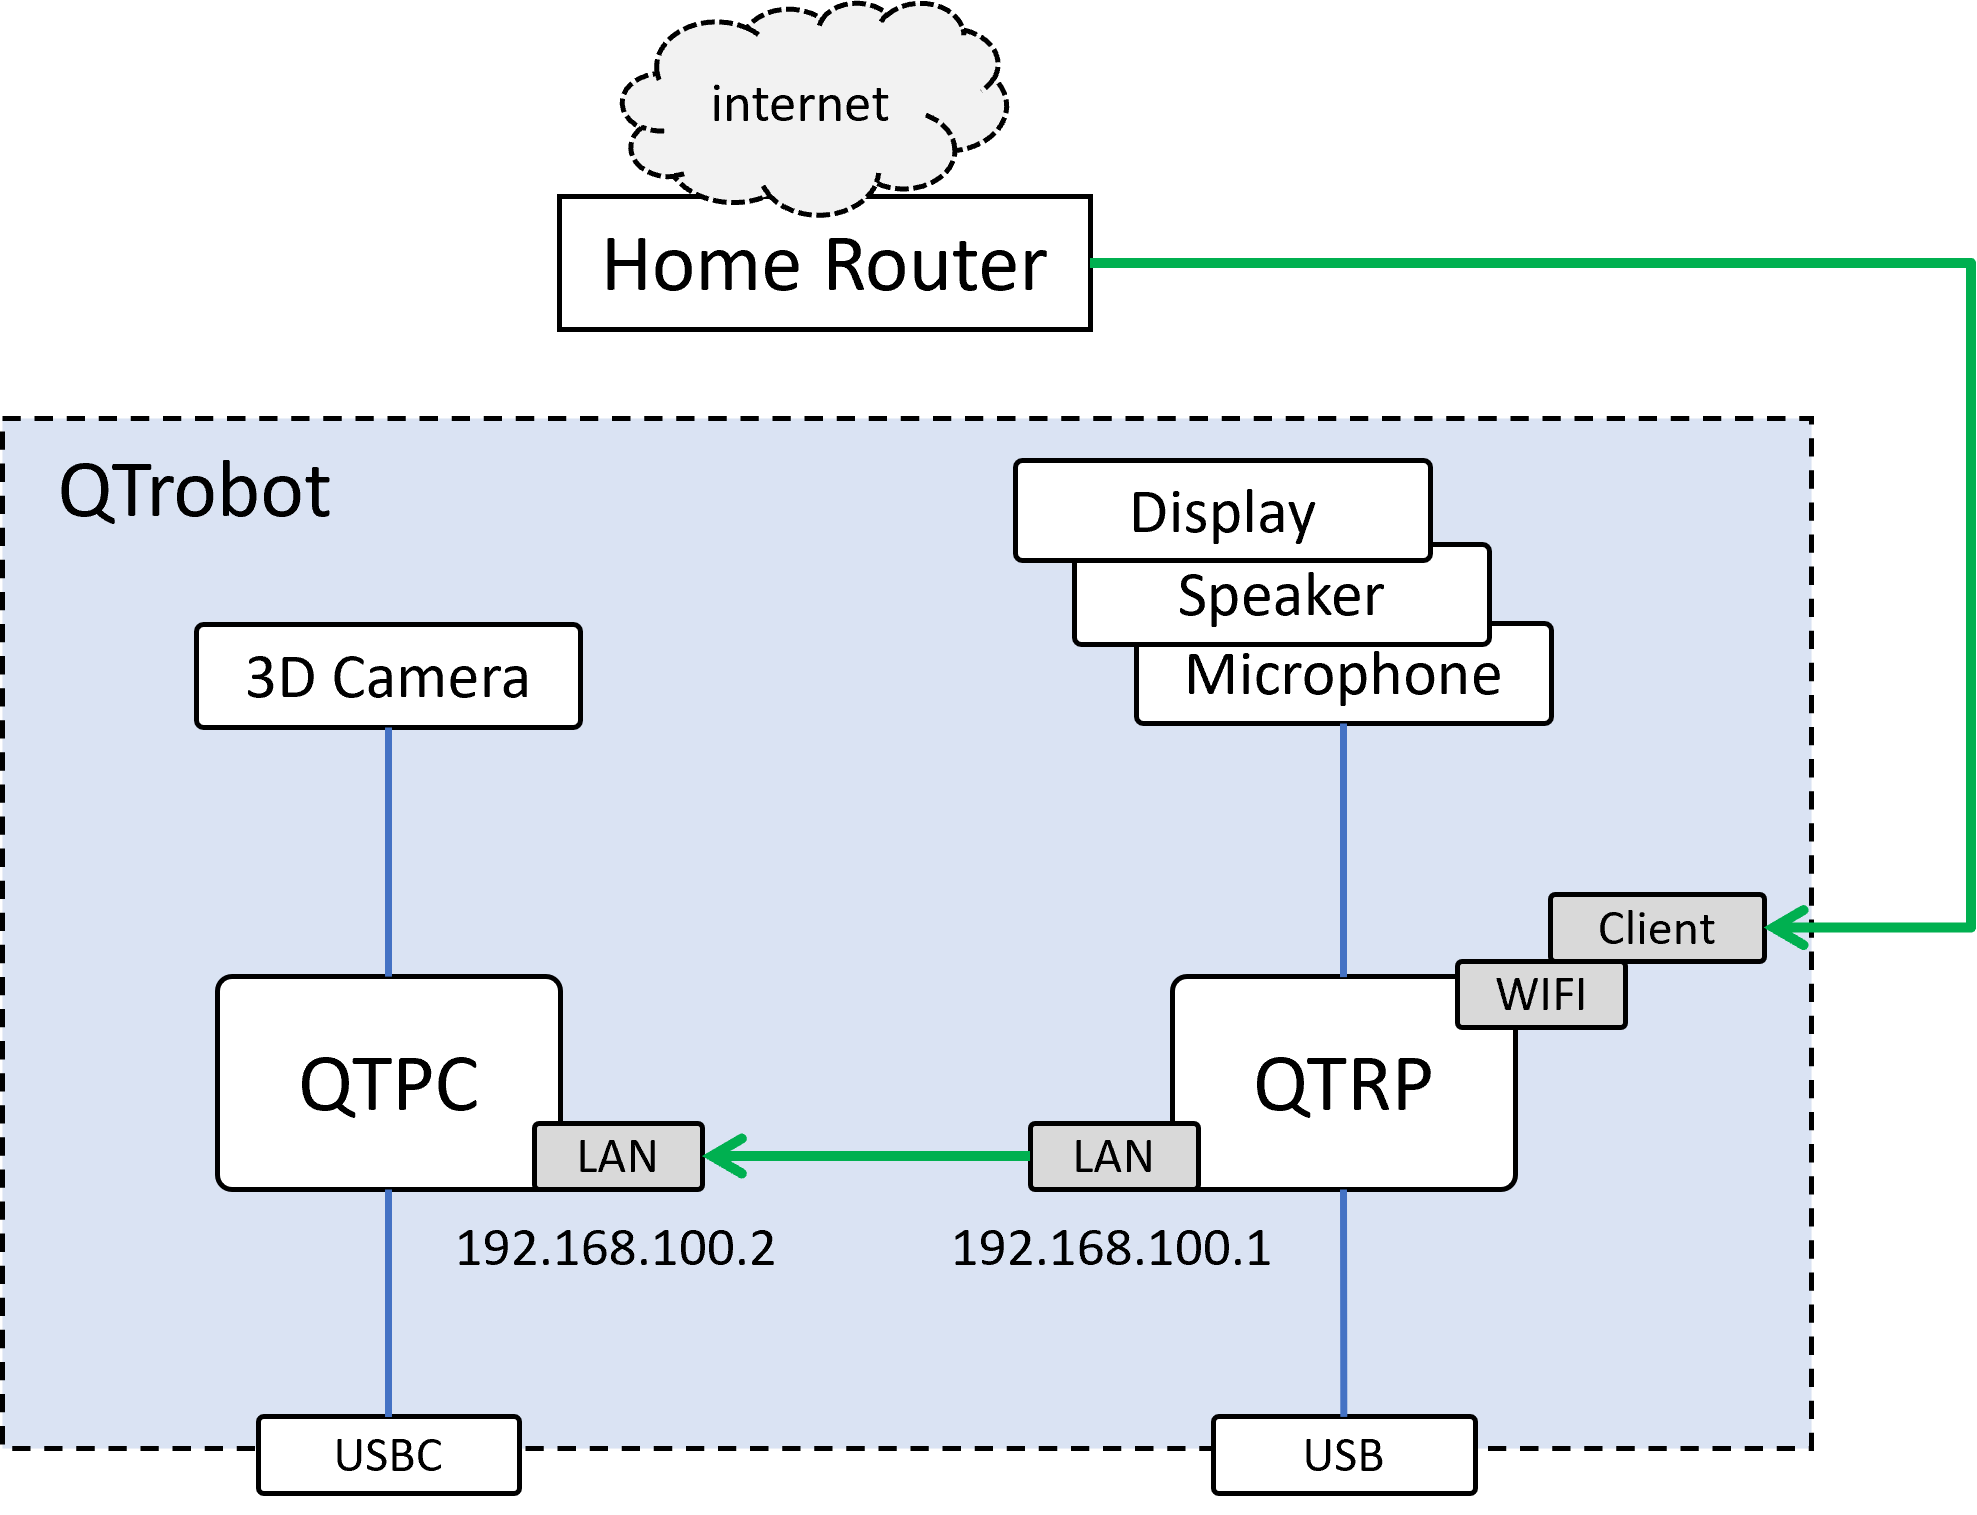
\includegraphics[width=0.85\textwidth]{figures/architecture_robot_network.png}
    \caption{Architecture réseau du QTRobot V2 en mode client~\cite{luxai_doc}.}
    \label{fig:archi_robot_network}
\end{figure}

Le robot utilisé en début de stage était en réalité un QTRobot V1, remplacé en cours de stage par ce QTRobot V2, pour deux raisons. D'une part, le V1 n'est plus maintenu par LuxAI, qui concentre désormais son support sur le V2. D'autre part, la communication entre le PC et le QTRP souffrait d'une latence perceptible sur le V1, imputable à son architecture réseau : le QTPC y disposait de sa propre connexion Wi-Fi vers le réseau externe, tandis que le QTRP gérait un point d'accès (hotspot) totalement indépendant, les deux fonctionnant sur des cartes Wi-Fi physiquement séparées et pouvant donc tourner simultanément sans conflit ; contrairement au V2, cette architecture ne contraignait pas les deux rôles à une seule carte partagée.

Le V2 présente par ailleurs plusieurs autres différences par rapport au V1. Le processeur embarqué est plus récent et plus puissant. Le réseau de microphones, basé sur du matériel de type ReSpeaker, gère mieux la suppression du bruit et la captation en champ lointain sur les révisions récentes. Les deux versions tournent toujours sous ROS\,1, mais sur des distributions différentes : Kinetic sous Python\,2.7 pour le V1, Noetic sous Python\,3 pour le V2. L'interface web accessible sur le V1 n'existe plus sur le V2. Enfin, les gestures et emotions préenregistrés ne sont pas exactement les mêmes d'une version à l'autre : certains sont propres au V1, d'autres au V2, sans qu'un ensemble soit strictement inclus dans l'autre.

\paragraph{Prise en main : fonctionnalités de base}

La connexion au robot s'effectue en SSH depuis le terminal d'un ordinateur vers le QTRP :

\begin{verbatim}
ssh developer@192.168.24.118
\end{verbatim}

L'ensemble des fonctionnalités du robot sont pilotées via des appels de services ROS. Les principaux services disponibles; parole, émotion, geste, volume, audio et behavior. Ces fonctionnalités suivent le format général suivant :

\begin{verbatim}
rosservice call /qt_robot/speech/say "message: '<TEXTE>'"
rosservice call /qt_robot/emotion/show "name: 'QT/<NOM_EMOTION>'"
rosservice call /qt_robot/gesture/play "name: 'QT/<NOM_GESTE>'"
rosservice call /qt_robot/setting/setVolume "volume: <VALEUR>"
rosservice call /qt_robot/audio/play "filename: 'QT/<FICHIER>'"
rosservice call /qt_robot/behavior/talkText "message: '<TEXTE>'"
\end{verbatim}

La <VALEUR> de volume est un entier compris entre 0 et 100. Les behaviors permettent de déclencher une séquence de parole avec animation de la bouche.

\subsubsection{Choix architecturaux}
\label{sec:architecture}

% Intro : avant d'aboutir à l'architecture finale, une première
% approche a consisté à garder toute l'intelligence sur le robot lui-même —
% utiliser son micro ReSpeaker et sa caméra intégrée. Cette piste a été
% abandonnée pour plusieurs raisons :
% (1) Qualité du micro : en présence de bruit ambiant, la reconnaissance
%     vocale était instable.
% (2) Dépendances Python 2 / Python 3 : tenter d'installer des libs récentes
%     sur le robot crée des conflits insolubles (voir ci-dessous, qt_vosk_app).
% (3) Caméra : fixée sur la tête de QT, elle ne peut pas photographier un
%     dessin posé sur une table sans que le participant ne le soulève.
% Solution retenue : externaliser les capteurs sur le PC (micro intégré du PC
% + caméra externe) et y concentrer toute l'intelligence du système.

\paragraph{Tentative initiale : capteurs embarqués sur le robot}

Le robot utilisé en début de stage était le QTRobot V1 (voir plus haut). La première difficulté rencontrée concerne la reconnaissance vocale. Le QTRobot V1 est censé embarquer \texttt{qt\_vosk\_app}, un module de reconnaissance vocale hors-ligne basé sur Vosk. Ce module était absent de la version du robot disponible au laboratoire. Une recherche a permis de retrouver une version du module publiée par LuxAI, mais celle-ci était conçue pour le QTRobot V2, qui fonctionne sous Python\,3, alors que le V1 tourne sous Python\,2. De nombreuses tentatives d'adaptation ont été menées, mais chacune se heurtait à des conflits de dépendances de bibliothèques insolubles : Vosk n'existe tout simplement pas pour Python\,2, et un pont Python\,2/Python\,3 aurait représenté une complexité injustifiée.

Face à cet échec, deux solutions alternatives ont été développées et exécutées directement sur le robot, en tirant parti de son microphone embarqué. L'extension Remote SSH de VS Code a été utilisée pendant cette phase pour éditer les fichiers directement dans le robot, tandis que la connexion SFTP (\texttt{sftp://qtrobot@192.168.100.1}) permettait de gérer les fichiers depuis le PC. La première solution, \texttt{ears.py}, tournait entièrement sur le robot et effectuait la reconnaissance vocale via la bibliothèque Python \texttt{speech\_recognition} et sa méthode \texttt{recognize\_google()}, qui transmet l'audio au service de reconnaissance Google sans clé API. La seconde, \texttt{ears\_v2.py}, tournait elle aussi sur le robot mais déportait le traitement : elle se contentait de capturer le flux audio du microphone et de l'envoyer vers le PC, où la reconnaissance était réalisée. Ces deux approches n'ont finalement pas donné de résultats satisfaisants : la reconnaissance restait peu fiable et la latence trop importante pour un usage en temps réel. Comme la caméra du robot devait de toute façon être remplacée par une caméra externe, le choix s'est porté sur une externalisation complète des capteurs, à commencer par un microphone externe branché sur le PC, pour garder davantage de contrôle sur toute la chaîne de traitement.

\paragraph{Solution retenue : externalisation sur le PC ROS\,2}

La solution retenue consiste à déporter l'ensemble du traitement, capteurs compris, sur un PC externe fonctionnant sous ROS\,2. Le microphone intégré du PC remplace celui du robot pour la reconnaissance vocale, et une caméra USB externe, positionnée au-dessus du participant, remplace la caméra embarquée pour photographier le dessin ; aucune caméra montée sur la tête du robot ne peut satisfaire correctement cette contrainte dans notre configuration d'expérience. Le robot lui-même ne conserve alors que ses fonctions d'expression : parole, gestes et émotions, pilotées à distance depuis le PC via le pont de communication décrit dans le paragraphe suivant.

Cette externalisation présente plusieurs avantages. Elle rend le système indépendant des limitations matérielles et logicielles propres au robot, comme celles rencontrées ci-dessus. Elle permet enfin de porter l'ensemble du système vers un autre QTRobot, quelle que soit sa version, sans aucune reconfiguration matérielle : seule la connexion réseau entre le PC et le robot doit être adaptée.

\subsubsection{Développement des composants}

Le système est organisé en trois couches : une couche logique qui pilote le déroulement de l'expérience (\texttt{orchestrator\_node}), une couche d'interaction qui traduit chaque phase en actions concrètes pour le robot (\texttt{interaction\_node}), et une couche de cognition qui regroupe l'intelligence artificielle et la perception (\texttt{brain\_node}, \texttt{stt\_node}, \texttt{vision\_node}, \texttt{drawing\_detector\_node}, \texttt{projection\_node}). Cette séparation rend le système modulaire : elle permet de modifier le timing, les phrases ou le comportement du modèle de langage sans avoir à toucher au reste du système, mais aussi d'adapter plus largement les phases et le déroulement de l'expérience, par exemple pour un protocole différent de celui de CreaRobot. Cette modularité est renforcée par la centralisation de la quasi-totalité des paramètres dans un unique fichier de configuration (\texttt{config.py}) : durées et seuils des différents mécanismes, phrases scriptées des conditions C0 et C2, et l'ensemble des prompts système utilisés par \texttt{brain\_node} pour C1, C2 et la détection d'adressage, tous reproduits en annexe. Ajuster le comportement du système, que ce soit un minuteur ou un prompt entier, ne nécessite ainsi de modifier qu'un seul fichier, sans toucher au code des nœuds eux-mêmes. La figure~\ref{fig:archi_systeme} présente l'ensemble de ces nœuds, tous exécutés côté PC (ROS\,2), leurs connexions, ainsi que leur liaison avec le matériel du robot (ROS\,1).

\begin{figure}[H]
    \centering
    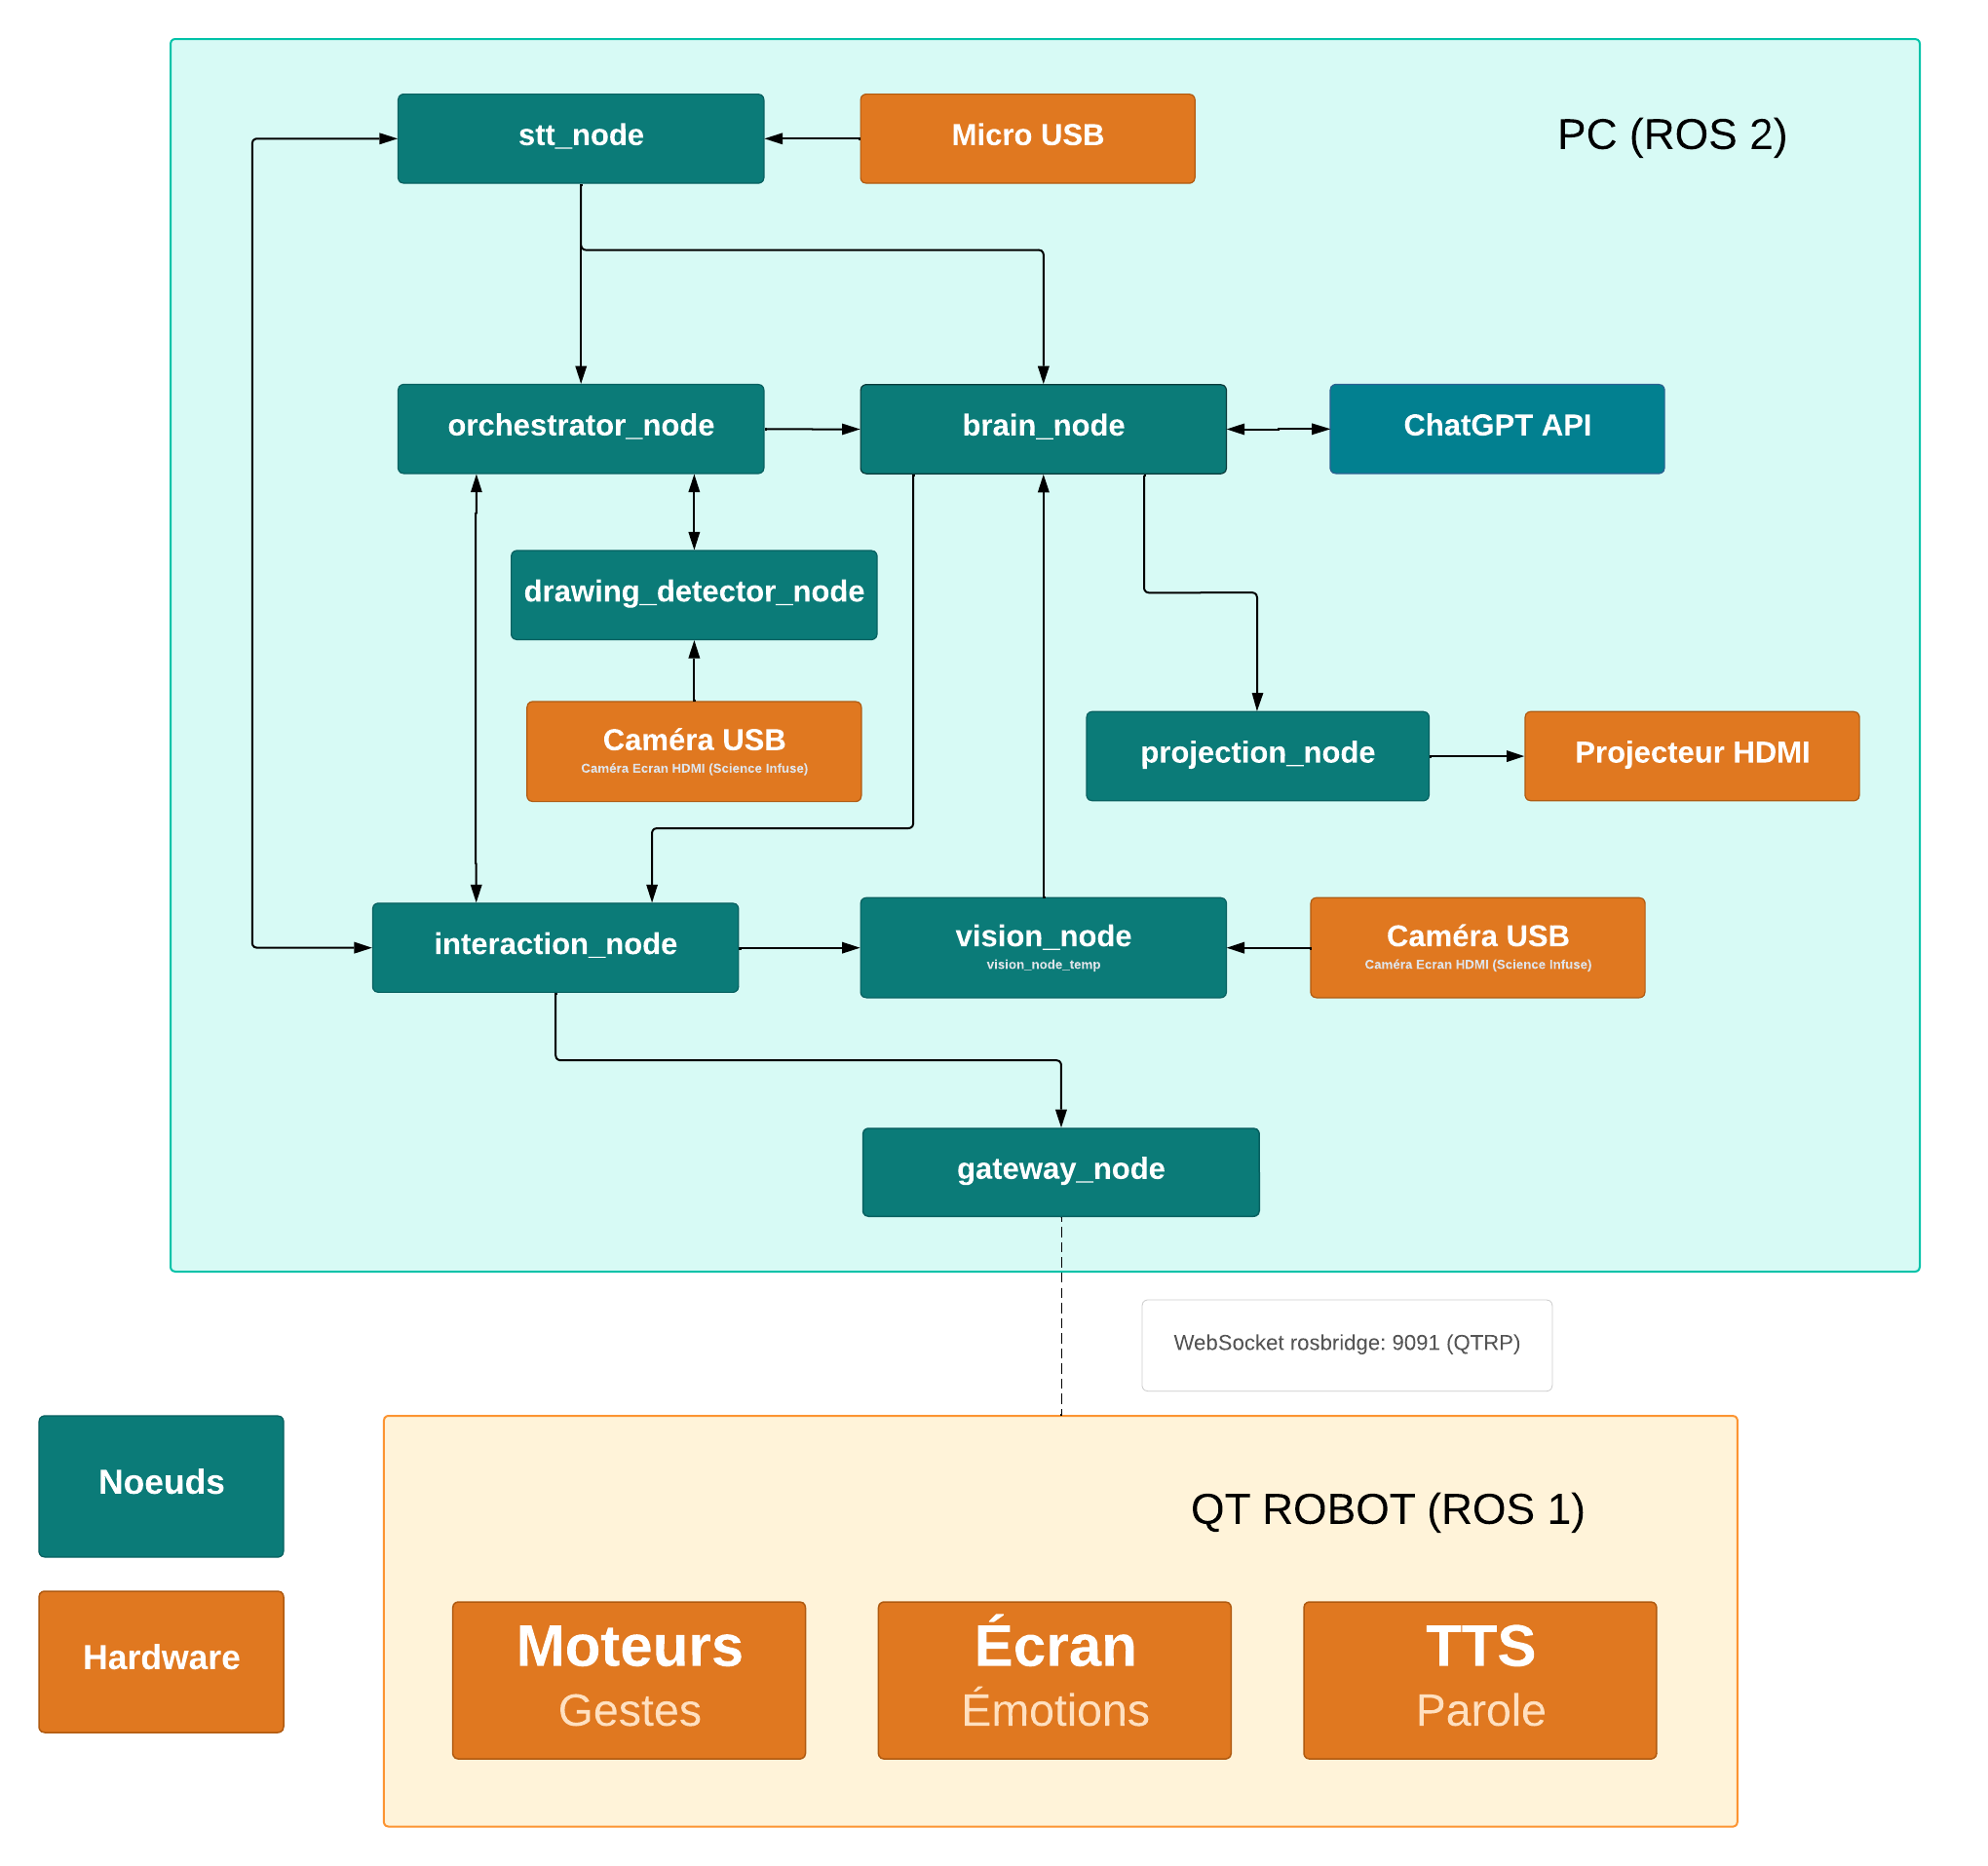
\includegraphics[width=\textwidth]{figures/architecture_système.png}
    \caption{Architecture logicielle du système CreaRobot : nœuds et répartition matérielle.}
    \label{fig:archi_systeme}
\end{figure}

Chaque nœud est détaillé ci-après dans l'ordre de la chaîne de décision : d'abord l'orchestrateur, qui décide de la phase en cours, puis l'interaction, qui la traduit en actions, puis le cerveau LLM, qui génère le contenu, puis la passerelle qui relaie tout cela au robot ; viennent ensuite les nœuds de perception, puis le système de lancement et la journalisation.

\paragraph{Le nœud orchestrateur (\texttt{orchestrator\_node})}

L'orchestrateur se situe au sommet de la hiérarchie logicielle : c'est lui qui pilote la machine à états représentant les sept phases de l'expérience (section~\ref{sec:protocole}) et qui décide, à tout moment, de la phase en cours et du tour de dessin. Il ne commande jamais directement le robot : il publie simplement la phase active sur \texttt{/pc/phase\_control} et le numéro de tour sur \texttt{/pc/tour\_control}, et ce sont les autres nœuds qui réagissent à ces publications.

Une transition de phase peut être déclenchée par plusieurs sources, qui diffèrent selon la phase en cours. Pendant l'introduction, elle est déclenchée par la détection d'un mot-clé (« oui », « prêt » ou « bon ») dans la transcription STT. Pendant la phase de dessin, quatre sources peuvent y mettre fin : un minuteur automatique (\texttt{DRAW\_DURATION} = 90\,s), un signal de fin de dessin envoyé par \texttt{drawing\_detector\_node}, un signal d'adressage envoyé par \texttt{brain\_node} lorsque le participant s'adresse au robot (prioritaire sur les deux précédents), ou une commande manuelle saisie dans le terminal (\texttt{fini}, \texttt{skip}, \texttt{terminate}, \texttt{title}), qui reste disponible à tout moment pour reprendre la main quelle que soit la phase. Pour toutes les autres phases (\texttt{ICE\_BREAKING}, \texttt{TASK\_INTRO}, \texttt{FEEDBACK}, \texttt{TITLE}), la transition suit simplement la fin normale de la phase, signalée par \texttt{interaction\_node} une fois celle-ci terminée. Un thread séparé, dédié à l'écoute du terminal, tourne en permanence aux côtés des minuteurs ; c'est pour cette raison que le nœud utilise un \texttt{MultiThreadedExecutor} plutôt que la boucle d'exécution standard de ROS\,2.

\paragraph{Le nœud d'interaction (\texttt{interaction\_node})}

Le nœud d'interaction reçoit les ordres de phase publiés par l'orchestrateur et les traduit en actions concrètes pour le robot : texte à prononcer, geste, émotion, et activation ou non du micro.

La phase \texttt{DRAWING} a un comportement plus spécifique que les autres : elle envoie une phrase d'encouragement différente selon le tour, oriente la tête selon un angle configurable (\texttt{HEAD\_PITCH\_DRAWING}, tête droite par défaut), ouvre le micro, et programme de petites animations aléatoires (toutes les 40 à 80 secondes) pour que le robot ne reste pas figé, la tête revenant à sa position de dessin quatre secondes après chaque animation.

La logique de la phase \texttt{FEEDBACK} dépend de la condition expérimentale : en C0, une phrase générique est tirée aléatoirement selon le tour, sans prise de photo ; en C1 et C2, une photo est prise en tout début de phase, précédée d'une courte phrase d'introduction ; si le tour a été interrompu par un adressage du participant, cette phrase a déjà été donnée par \texttt{brain\_node} au moment de la détection (voir le paragraphe qui lui est consacré ci-après), et n'est donc pas répétée ici. L'échange C1 se poursuit ensuite sur trois tours au maximum, tandis que le feedback C2 affiche une phrase d'invitation à s'inspirer une fois l'image générée reçue. Cette prise de photo, comme celle de la phase \texttt{TITLE}, se fait en publiant sur le topic \texttt{/pc/camera/trigger}, que \texttt{vision\_node} écoute pour déclencher la capture (voir plus loin). 

Le nœud contrôle également l'activation du micro selon la phase, via le topic \texttt{/pc/stt/enable} : c'est lui qui décide, à chaque instant, si une réponse du participant est attendue ou non (le verrouillage complet, incluant le silence du robot pendant qu'il parle, est détaillé dans le paragraphe consacré à \texttt{stt\_node}). Il gère aussi une relance automatique en cas de silence prolongé du participant. Pour enchaîner ses propres actions (rouvrir le micro, déclencher la photo, passer à la phase suivante) au bon moment, il s'abonne au signal réel \texttt{/pc/robot/speaking} publié par \texttt{gateway\_node} (voir plus bas) et attend que le robot ait effectivement fini de parler.

\paragraph{Le nœud d'intelligence artificielle (\texttt{brain\_node})}
\label{sec:brain_node}

Le \texttt{brain\_node} concentre l'intelligence artificielle du système, via l'API OpenAI : GPT-4o-mini pour tout ce qui est textuel et vision, et gpt-image-1.5 pour la génération d'image en C2. Il assure quatre fonctions principales : détecter en temps réel un adressage spontané du participant pendant qu'il dessine, décrire le dessin au fil des tours, générer les réponses du robot en condition C1, et produire l'image augmentée en condition C2.

Pendant la phase \texttt{DRAWING}, chaque transcription STT est analysée dans un thread séparé pour déterminer si le participant s'adresse au robot. Si c'est le cas et que la phase n'a pas changé entretemps, le nœud envoie immédiatement une courte réponse à l'aveugle et publie un signal sur \texttt{/pc/brain/addressing\_detected}, que l'orchestrateur utilise pour interrompre le minuteur de dessin en cours ; la phrase du participant est mémorisée pour être réintégrée dans le prochain prompt de feedback. Si une nouvelle transcription arrive pendant qu'une vérification est en cours, seule la plus récente est traitée.

À chaque photo reçue, le nœud maintient une mémoire visuelle cumulative du dessin : la première photo produit une description complète, chaque photo suivante ne décrit que ce qui a changé, le tout étant concaténé plutôt que de redemander une description complète à chaque fois. En condition C1, le nœud déclenche alors la génération d'une réponse, construite à partir du prompt système (section~\ref{sec:condition_c1}), de l'historique de la conversation et de cette mémoire visuelle. Si le participant s'était adressé au robot juste avant la photo, sa phrase aurait été intégrée au prompt pour que la réponse en tienne compte.

En condition C2, la photo reçue déclenche un traitement différent : une description de l'intention du participant est d'abord produite (\texttt{PROMPT\_C2\_ANALYSIS}, reproduit en annexe~\ref{annexe:prompt_c2_analysis}), puis transmise avec le dessin et la feuille TCT-DP vierge de référence (section~\ref{sec:tctdp_description}) à gpt-image-1.5, qui génère une version augmentée. L'image obtenue est redimensionnée puis publiée pour \texttt{projection\_node} (voir plus bas) ; le robot prononce ensuite une courte phrase annonçant sa proposition, adaptée selon qu'un adressage a eu lieu ou non juste avant.

Pendant les phases \texttt{FEEDBACK} (C1) et \texttt{ICE\_BREAKING}, chaque nouvelle réponse du participant relance un appel au modèle de langage : le message envoyé combine le prompt système de la phase en cours (\texttt{PROMPT\_C1} ou \texttt{PROMPT\_ICE\_BREAKING} selon le cas), les \texttt{HISTORY\_LIMIT} derniers échanges de l'historique (paramètre de \texttt{config.py}, fixé à trois par défaut), et la réponse du participant. Un indicateur (\texttt{\_c1\_ready}) empêche qu'une transcription arrivée trop tôt ne soit comptée comme un échange valide avant que la première réponse du tour n'ait été générée.

Enfin, \texttt{brain\_node} tient le journal de chaque session (voir plus loin) et envoie un appel de chauffe au démarrage vers GPT-4o-mini, et vers gpt-image-1.5 en condition C2, pour absorber la latence de démarrage (jusqu'à une minute pour le premier appel d'image) avant le premier vrai feedback.

\paragraph{Le nœud Gateway (\texttt{gateway\_node})}

Le rosbridge du QTRobot V1 était un simple pont WebSocket, accessible sans authentification. Sur le V2, le rosbridge actif par défaut impose une authentification HMAC via le service \texttt{/authenticate} (\texttt{rosauth}), non supportée par la bibliothèque roslibpy utilisée par \texttt{gateway\_node} pour communiquer avec le robot. Une seconde instance de rosbridge, sans SSL ni authentification, a donc été lancée sur QTRP sur un port dédié (9091) (solution recommandée par la documentation LuxAI pour ce cas de figure), intégrée à l'autostart du robot pour être disponible à chaque démarrage. C'est ce second rosbridge que \texttt{gateway\_node} utilise pour se connecter au robot.

Une fois connecté, \texttt{gateway\_node} configure automatiquement la langue et le volume de la voix du robot à partir de \texttt{config.py}, puis agit comme traducteur universel entre le reste du système et les services ROS\,1 du robot : il écoute le topic \texttt{/pc/qtaction} (un triplet JSON \texttt{[geste, emotion, texte]}) et déclenche les appels de service correspondants. Trois cas sont distingués : un texte seul déclenche directement le behavior de parole du robot, qui anime aussi la bouche en synchronisation (plutôt qu'un simple service de synthèse vocale) ; un geste ou une émotion sans texte est joué immédiatement ; et lorsque texte, geste et émotion sont combinés, ce même behavior de parole est lancé en parallèle avec les appels de geste et d'émotion via un synchroniseur dédié (\texttt{TaskSynchronizer}, basé sur \texttt{asyncio}). Il relaie par ailleurs séparément les commandes d'orientation de la tête reçues d'\texttt{interaction\_node}, et publie un indicateur \texttt{/pc/robot/speaking} pendant qu'il parle, utilisé par \texttt{stt\_node} (voir plus bas) pour éviter que le robot ne s'écoute lui-même.

\paragraph{Le nœud de reconnaissance vocale (\texttt{stt\_node})}

Le nœud de reconnaissance vocale tourne sur le PC et utilise son micro intégré (ou un micro externe, au choix) plutôt que celui du robot (voir section~\ref{sec:architecture}). Il repose sur Faster-Whisper, modèle \texttt{small} sur GPU (CUDA, \texttt{float16}), avec un repli automatique sur le modèle \texttt{base} en CPU (\texttt{int8}) si aucun GPU n'est disponible. L'audio est capturé en continu, mais n'est transcrit et publié que lorsque deux conditions sont réunies : le micro a été activé par \texttt{interaction\_node} via le topic \texttt{/pc/stt/enable}, et le robot n'est pas lui-même en train de parler, signalé par \texttt{gateway\_node} sur \texttt{/pc/robot/speaking}. Ce second signal implémente un verrouillage demi-duplex : dès que \texttt{gateway\_node} lance un appel de parole, il publie \texttt{True} sur ce topic, ce qui vide immédiatement le tampon audio de \texttt{stt\_node} et suspend l'écoute, avant de republier \texttt{False} une fois la phrase terminée pour la réactiver ; ce mécanisme évite que le robot ne capte sa propre voix et ne s'y réponde. Une transcription n'est publiée qu'après au moins 0,9\,seconde de silence en fin de tampon audio, ce qui laisse au participant le temps de terminer sa phrase sans la couper prématurément. Un filtre écarte enfin certaines hallucinations connues de Whisper : le texte transcrit est comparé à une liste de formulations récurrentes observées (mentions de sous-titrage, incitations à s'abonner, etc.), et la transcription est écartée si elle en contient une.

\paragraph{Le nœud de vision (\texttt{vision\_node})}

\texttt{vision\_node} photographie le dessin du participant via une caméra USB externe (voir section~\ref{sec:architecture}) : il attend un déclenchement sur le topic \texttt{/pc/camera/trigger} (publié par \texttt{interaction\_node}, voir plus haut), ouvre la caméra, vide les cinq premières frames du tampon pour garantir une image à jour, capture, puis relâche immédiatement la caméra. La photo est encodée en JPEG base64 et publiée pour \texttt{brain\_node} ; son enregistrement dans le dossier de la session est décrit plus loin, dans la partie consacrée à la journalisation.

Une variante, \texttt{vision\_node\_temp}, capture un écran HDMI externe plutôt qu'une caméra ; elle a été développée pour la Semaine de la Science Infuse (voir section~\ref{sec:scienceinfuse}).

\paragraph{Le nœud de détection de fin de dessin (\texttt{drawing\_detector\_node})}
\label{sec:drawing_detector}

Pour savoir quand un participant a fini de dessiner sans le lui demander explicitement, le timer fixe (\texttt{DRAW\_DURATION} = 90\,s) reste le mécanisme principal, mais un mécanisme complémentaire permet de terminer la phase plus tôt si le participant a clairement arrêté. L'approche retenue est un frame differencing à médiane glissante : à chaque tick (1\,s), deux frames consécutives de la caméra sont comparées pixel à pixel, et le nombre de pixels différents est ajouté à une fenêtre glissante de six valeurs. Si la médiane de cette fenêtre reste sous un seuil pendant six secondes, un signal de fin de dessin est publié sur le topic \texttt{/pc/vision/drawing\_stopped}, que l'orchestrateur écoute pour faire passer l'expérience à la phase suivante, comme si le minuteur avait expiré. La détection ne s'active en réalité que 20 secondes après le début de la phase de dessin, pour laisser au participant le temps de réfléchir à ce qu'il va dessiner avant de commencer, sans que cette immobilité initiale ne soit interprétée comme une fin de dessin. Utiliser la médiane sur cette fenêtre, plutôt que la seule dernière valeur, évite qu'un pic isolé (changement de lumière, micro-mouvement) ne réinitialise à tort le compteur d'inactivité.

La limite principale de cette approche est qu'elle ne distingue pas un participant qui réfléchit, la main immobile dans le cadre, d'un participant qui a réellement terminé : les deux cas produisent une différence d'image tout aussi faible, et peuvent donc déclencher à tort la fin de la phase de dessin après six secondes d'immobilité. Un masquage par couleur de peau ou un comptage des pixels très sombres ont été envisagés pour mieux distinguer ces cas, mais rien ne garantissait leur fiabilité et il aurait fallu de nombreux tests pour le vérifier, un temps que la fin du stage ne permettait plus. Le nœud n'ouvre la caméra que pendant la phase de dessin et la libère immédiatement après, en vidant systématiquement le tampon interne d'OpenCV avant chaque capture pour garantir une frame à jour.

\paragraph{Le nœud de projection (\texttt{projection\_node})}

Le nœud de projection reçoit sur le topic \texttt{/pc/projector/image} les images publiées par \texttt{brain\_node} et les affiche en plein écran via OpenCV. Le projecteur est détecté automatiquement via \texttt{xrandr} ; en son absence, la fenêtre s'affiche simplement sur l'écran principal. L'enregistrement de chaque image reçue est décrit plus loin, dans la partie consacrée à la journalisation. L'image reste affichée pendant une durée configurable (\texttt{PROJECTION\_DISPLAY\_DURATION}), après quoi l'écran revient à un fond blanc ; ce minuteur est indépendant du reste du système et n'influence pas la transition vers la phase suivante, gérée séparément par \texttt{orchestrator\_node}.

\paragraph{Système de lancement (\texttt{launch.py})}

Le launch file démarre en une seule commande les nœuds \texttt{gateway\_node}, \texttt{stt\_node}, \texttt{interaction\_node}, \texttt{brain\_node}, \texttt{vision\_node} et \texttt{drawing\_detector\_node}. Le nœud de projection y est ajouté automatiquement si la condition active est C2 :

\begin{verbatim}
ros2 launch crearobot_brain launch.py
\end{verbatim}

L'orchestrateur, qui pilote manuellement le déroulement de l'expérience depuis le terminal, est volontairement lancé à part, dans un second terminal dédié : cela garde ses logs séparés de ceux des autres nœuds pour plus de clarté, et facilite le pilotage manuel, notamment lors des tests, où il est pratique de pouvoir sauter ou forcer une phase directement depuis ce terminal (commandes présentées plus haut).

\begin{verbatim}
ros2 run crearobot_brain orchestrator
\end{verbatim}

\paragraph{Journalisation automatique des sessions expérimentales}
\label{sec:logging}

Chaque session s'appuie sur un même dossier horodaté (\texttt{crearobot\_sessions/AAAA-MM-JJ/HH-MM-SS/}), créé au démarrage par \texttt{brain\_node} (voir plus haut) et transmis aux autres nœuds concernés via le topic latché \texttt{/pc/session\_dir}. Ce dossier réunit trois éléments, détaillés dans le tableau~\ref{tab:session_structure} : un fichier \texttt{conversation.log}, et deux sous-dossiers d'images, \texttt{dessins/} et \texttt{dessins\_generes/}.

\texttt{brain\_node} écrit lui-même le fichier \texttt{conversation.log} : chaque ligne est horodatée et préfixée par un mot-clé : \texttt{PARTICIPANT} pour les transcriptions STT, \texttt{ROBOT} pour le texte prononcé par le robot, et \texttt{PHASE} pour chaque transition d'état, cette dernière incluant le numéro de tour et, pour les sorties de la phase de dessin, la cause de la transition (adressage détecté, minuteur expiré, inactivité détectée par frame differencing, ou commande manuelle depuis le terminal).

Les deux sous-dossiers, eux, sont remplis séparément par \texttt{vision\_node} et \texttt{projection\_node}, pour y ranger respectivement les photos du dessin réel et les images générées en condition C2, chaque fichier étant nommé avec son index, la phase, le tour et l'heure exacte.

\begin{table}[H]
    \centering
    \renewcommand{\arraystretch}{1.6}
    \begin{tabular}{@{}lp{8.5cm}@{}}
        \toprule
        \textbf{Chemin} & \textbf{Contenu} \\
        \midrule
        \texttt{crearobot\_sessions/AAAA-MM-JJ/HH-MM-SS/} & Dossier horodaté de la session, créé au démarrage par \texttt{brain\_node} \\
        \texttt{conversation.log} & Transcriptions \texttt{PARTICIPANT}, textes \texttt{ROBOT} et transitions de \texttt{PHASE} \\
        \texttt{dessins/} & Photos du dessin réel, prises par \texttt{vision\_node} (ex. \texttt{01\_feedback\_tour1\_14-33-12.jpg}) \\
        \texttt{dessins\_generes/} & Images générées par IA et projetées en condition C2, sauvegardées par \texttt{projection\_node} (ex. \texttt{01\_genere\_14-33-55.jpg}) \\
        \bottomrule
    \end{tabular}
    \renewcommand{\arraystretch}{1}
    \caption{Structure du dossier créé pour chaque session.}
    \label{tab:session_structure}
\end{table}

\newpage

\subsection{Déroulement de la passation pilote : Semaine de la Science Infuse}
\label{sec:scienceinfuse}

\subsubsection{Contexte et objectifs de cette phase pilote}

Cette première passation s'est déroulée à la Cité des Sciences et de l'Industrie, à Paris, dans le cadre de la Semaine de la Science Infuse, un événement public d'une semaine organisé chaque année (édition d'avril 2026 pour cette passation). Elle poursuivait trois objectifs : obtenir de premiers résultats préliminaires, mener une étude exploratoire à partir des données recueillies, et tester le système en conditions réelles, avec des participants de passage plutôt que recrutés spécifiquement pour l'étude. Ces conditions restaient cependant éloignées de celles, plus contrôlées, envisagées pour la passation principale (voir les limites de l'étude exploratoire, section~\ref{sec:limites}). Cette passation s'est déroulée avec le QTRobot V1, avant son remplacement par le V2 (voir section~\ref{sec:qtrobot}).

\subsubsection{Déroulement}

La figure~\ref{fig:science_infuse} illustre le dispositif mis en place sur le stand : une participante en train de dessiner, le robot QT, la caméra utilisée pour capturer le dessin, la feuille TCT-DP, et un écran diffusant en direct le dessin du participant pour les visiteurs autour du stand.

\begin{figure}[H]
    \centering
    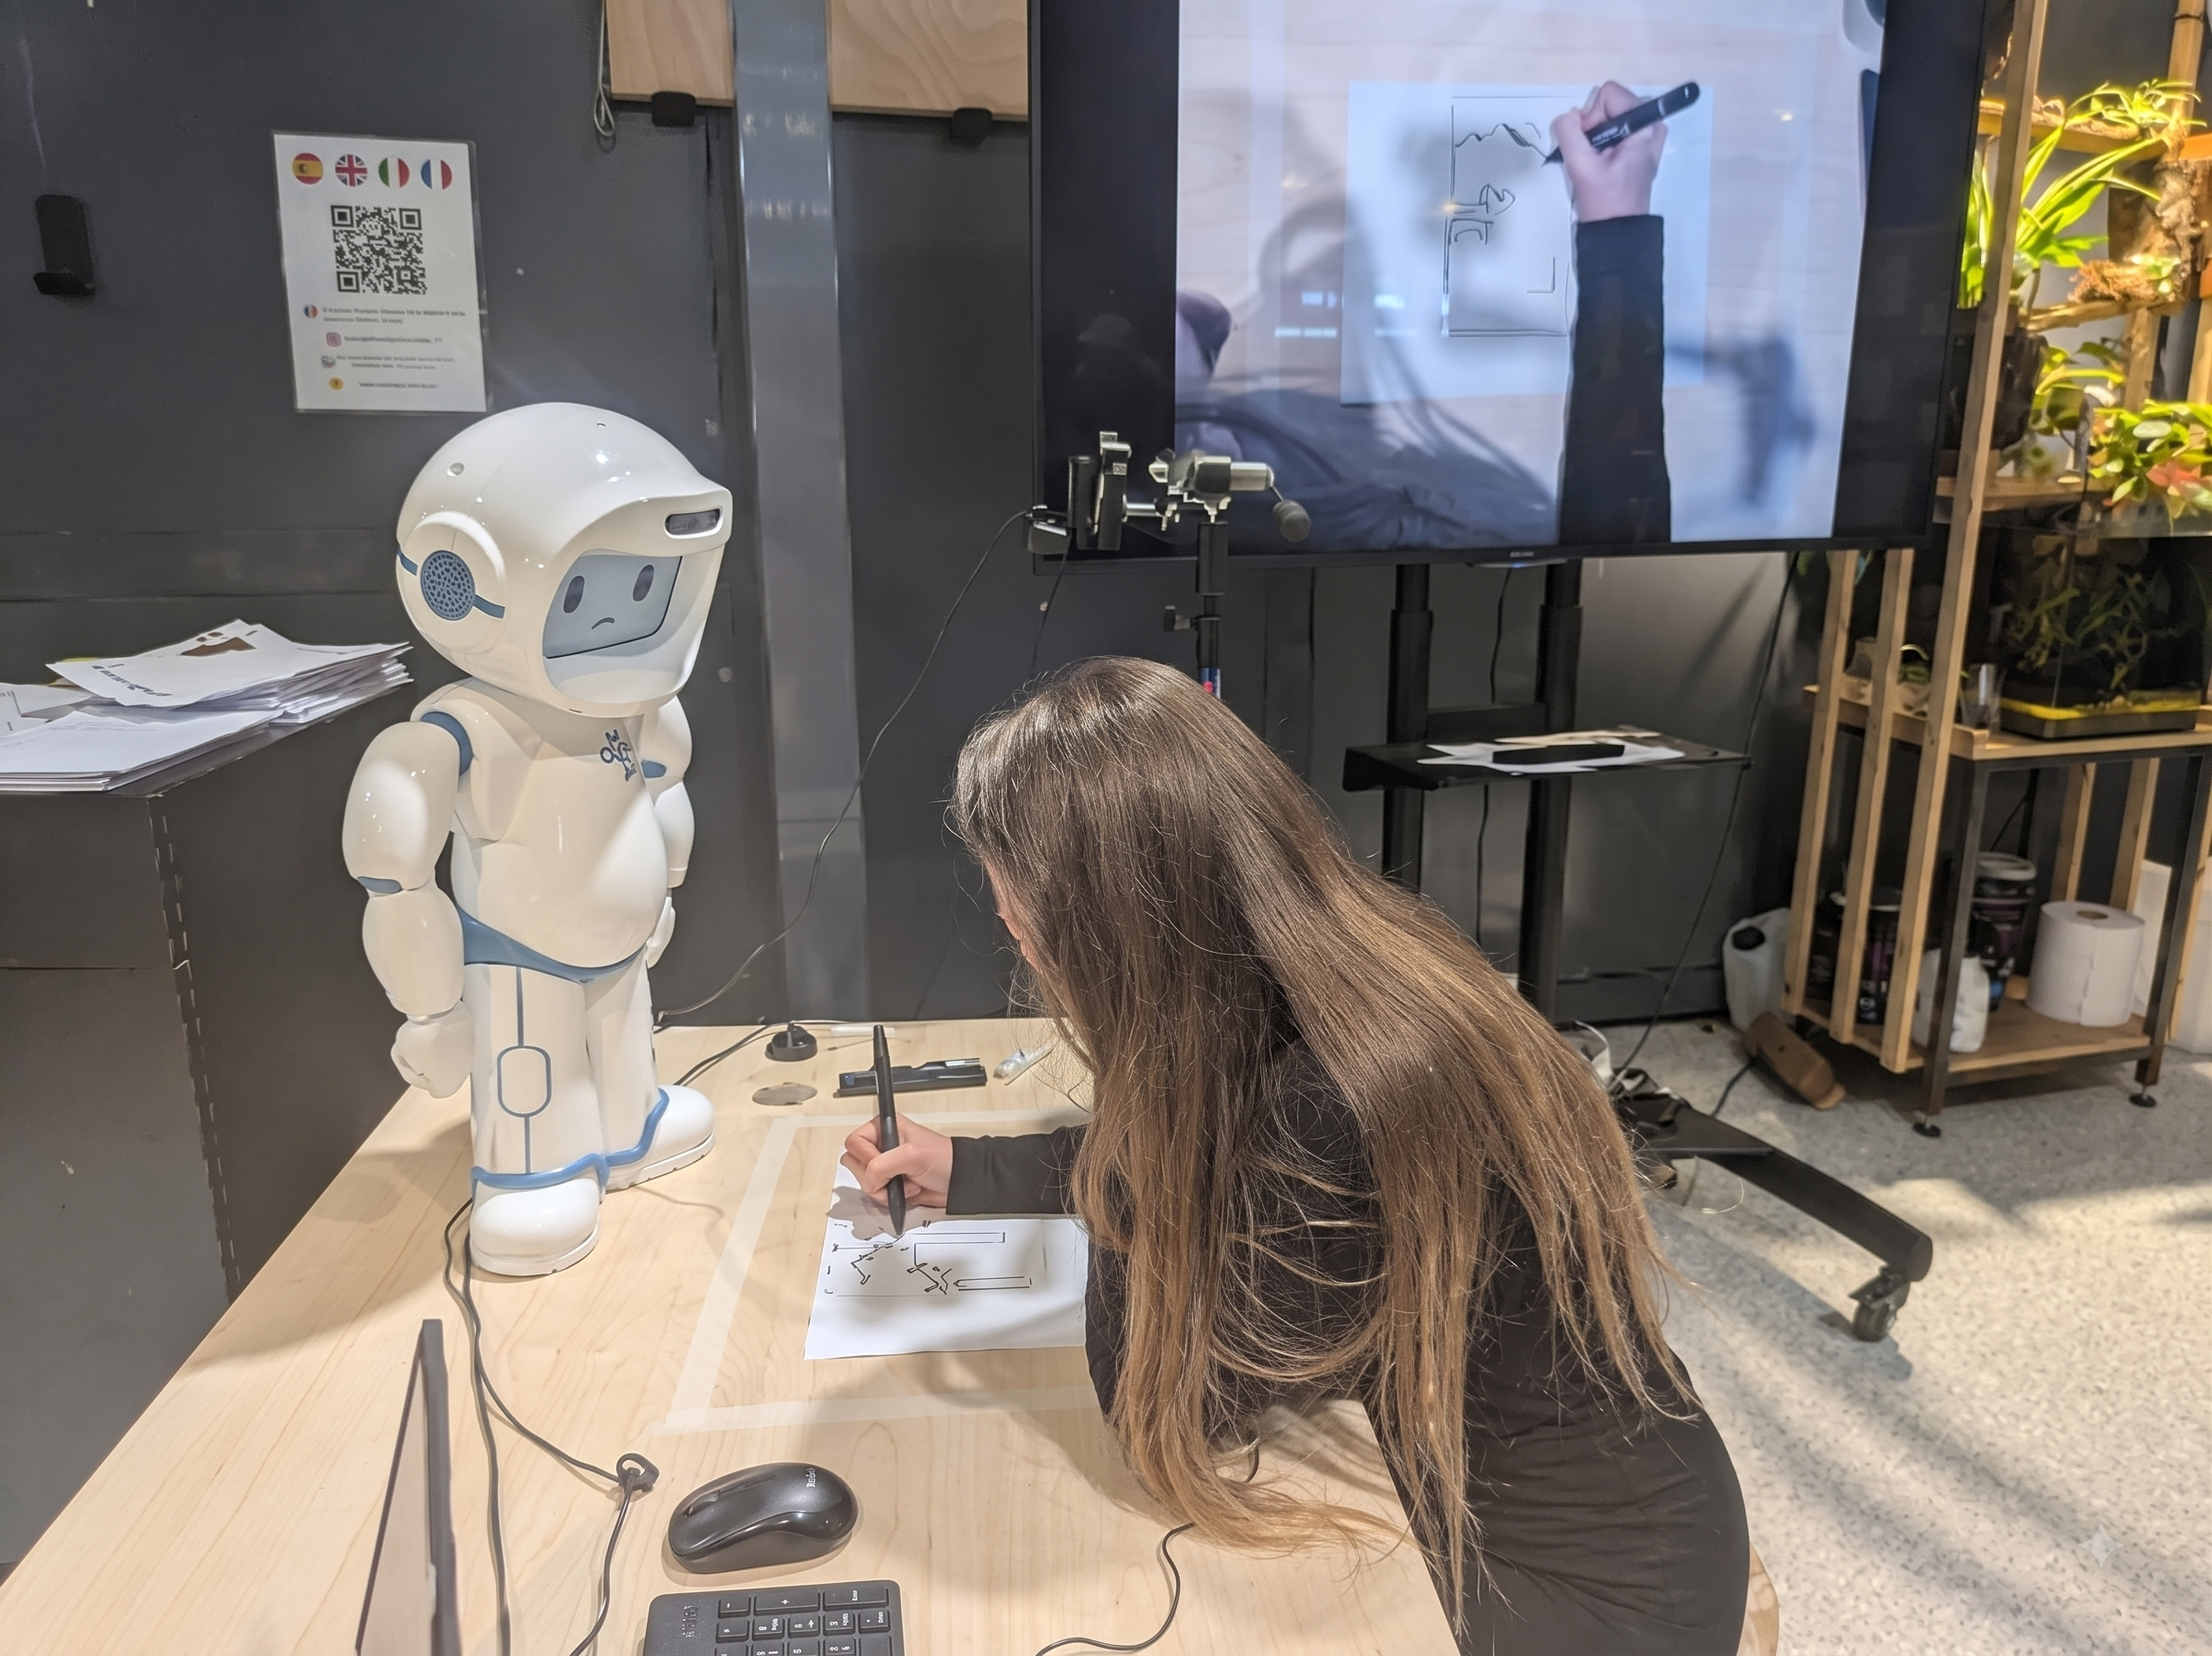
\includegraphics[width=0.85\textwidth]{figures/photo_science_infuse.png}
    \caption{Dispositif de passation lors de la Semaine de la Science Infuse (avril 2026).}
    \label{fig:science_infuse}
\end{figure}

La passation s'est déroulée sur trois jours, chaque session durant environ dix minutes. Cinquante-sept sessions ont été enregistrées, dont huit ont été exclues, certaines en raison d'interruptions techniques et d'autres parce que le participant dépassait la tranche d'âge visée, portant l'échantillon final à 49 participants : 26 en condition C0 et 23 en condition C1 (la condition C2 n'a pas été testée lors de cette passation pilote). La population était composée d'enfants âgés de 5 à 15 ans. Les données recueillies pour chaque session comprenaient les logs du terminal, enregistrés manuellement (le mécanisme de journalisation automatique décrit plus haut n'existait pas encore), la photo du dessin final uniquement (les photos prises à chaque tour de feedback n'étaient, elles, pas encore enregistrées), et des notes d'observation qualitative prises en direct par les expérimentateurs sur l'attitude du participant et ses interactions avec le robot et son entourage.

La cotation des dessins a été réalisée par Marco Grandclaude et Claudie Cuveillier, en aveugle par rapport à la condition expérimentale : au moment de noter un dessin, les deux évaluateurs ignoraient s'il provenait de la condition C0 ou C1. La notation s'est faite à deux simultanément plutôt qu'indépendamment : pour chaque critère, chaque évaluateur annonce son score, et en cas de désaccord, les deux se concertent jusqu'à trouver un accord commun.

\newpage

% ============================================================
\section{Résultats}

\subsection{Déroulement illustré de l'expérience}

En complément de la description technique des sept phases de l'expérience (section~\ref{sec:protocole}, figure~\ref{fig:session}), la figure~\ref{fig:bd_experience} illustre, sous forme de bande dessinée, le déroulement concret d'une session pour un participant fictif, en condition C1. Le cycle \texttt{DRAWING}/\texttt{FEEDBACK} se répète jusqu'à trois fois avant la phase \texttt{TITLE}, chaque tour de dessin étant suivi d'un échange sur le dessin en cours.

\newcommand{\bdcase}[2]{%
    \begin{minipage}[b]{#1}
        \centering
        \includegraphics[width=\textwidth]{#2}
    \end{minipage}%
}

\begin{figure}[H]
    \centering

    \bdcase{0.49\textwidth}{figures/bd_intro.png}%
    \hspace{1mm}%
    \bdcase{0.49\textwidth}{figures/bd_ice_breaking.png}

    \vspace{2mm}

    \bdcase{0.49\textwidth}{figures/bd_task_intro.png}%
    \hspace{1mm}%
    \bdcase{0.49\textwidth}{figures/bd_drawing.png}

    \vspace{2mm}

    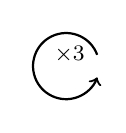
\begin{tikzpicture}
        \draw[->, thick] (0.5,0.4) arc[start angle=20, end angle=340, radius=0.42cm];
        \node at (0.15,0.4) {\footnotesize $\times 3$};
    \end{tikzpicture}

    \vspace{2mm}

    \bdcase{0.49\textwidth}{figures/bd_feedback.png}%
    \hspace{1mm}%
    \bdcase{0.49\textwidth}{figures/bd_title.png}

    \vspace{2mm}

    \bdcase{0.49\textwidth}{figures/bd_ending.png}

    \caption{Déroulement illustré d'une session type, en condition C1 (\texttt{INTRO}, \texttt{ICE\_BREAKING}, \texttt{TASK\_INTRO}, puis le cycle \texttt{DRAWING}/\texttt{FEEDBACK} répété jusqu'à trois fois, \texttt{TITLE} et \texttt{ENDING}).}
    \label{fig:bd_experience}
\end{figure}

\subsection{Évolution du dessin en cours de session}

Les figures~\ref{fig:evolution_c1} et~\ref{fig:evolution_c2} montrent, pour une session C1 et une session C2, l'évolution du même dessin au fil des trois tours, chaque photo correspondant au moment où \texttt{vision\_node} capture la feuille (fin de tour 1, fin de tour 2, puis la photo finale de la phase \texttt{TITLE}). Cette progression n'est pas montrée pour la condition C0 : les feedbacks y étant génériques et non liés au contenu du dessin, seule la photo finale était enregistrée pour cette condition lors de cette passation pilote.

\begin{figure}[H]
    \centering
    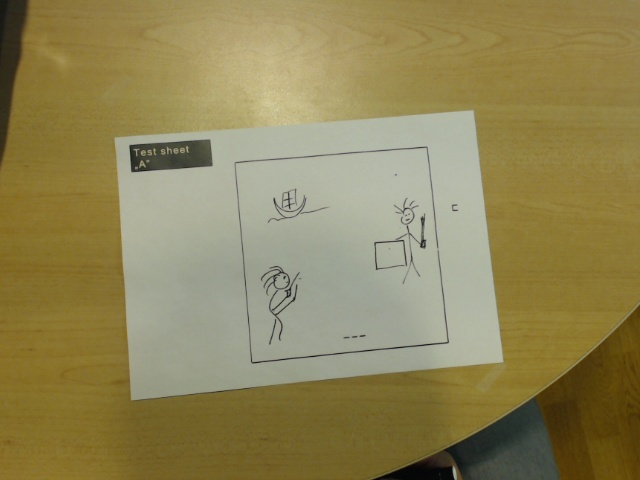
\includegraphics[width=0.32\textwidth]{figures/evolution_c1_tour1.jpg}\hfill
    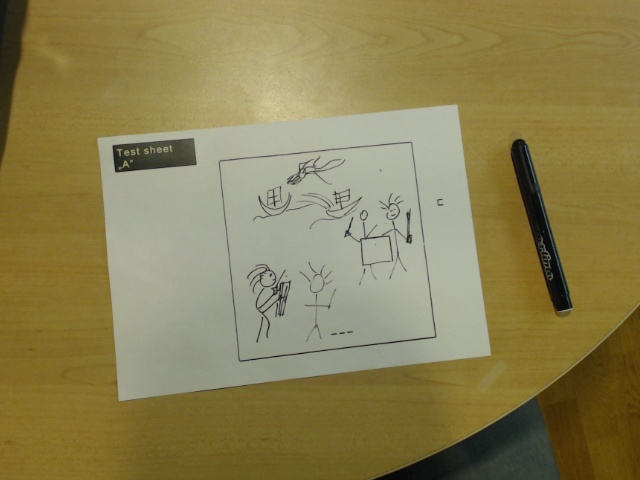
\includegraphics[width=0.32\textwidth]{figures/evolution_c1_tour2.jpg}\hfill
    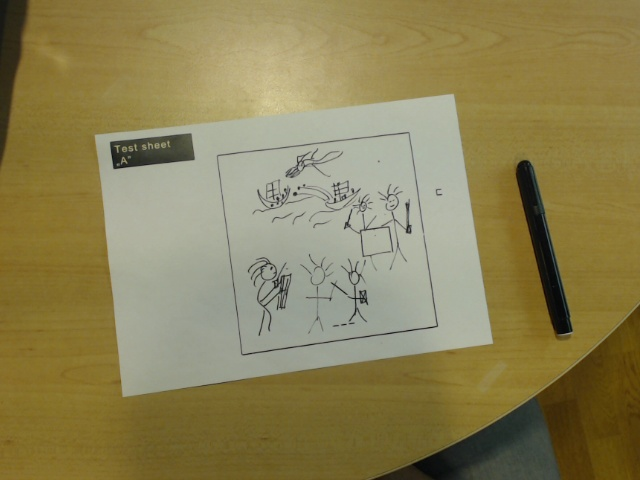
\includegraphics[width=0.32\textwidth]{figures/evolution_c1_tour3.jpg}
    \caption{Évolution d'un dessin sur les trois tours, en condition C1 (de gauche à droite : fin de tour 1, fin de tour 2, dessin final).}
    \label{fig:evolution_c1}
\end{figure}

En condition C2, le dessin réel du participant (figure~\ref{fig:evolution_c2}) est accompagné à chaque tour d'une proposition visuelle générée par gpt-image-1.5 à partir de ce même dessin (figure~\ref{fig:evolution_c2_genere}), que le participant peut ensuite choisir de reprendre ou d'ignorer au tour suivant.

\begin{figure}[H]
    \centering
    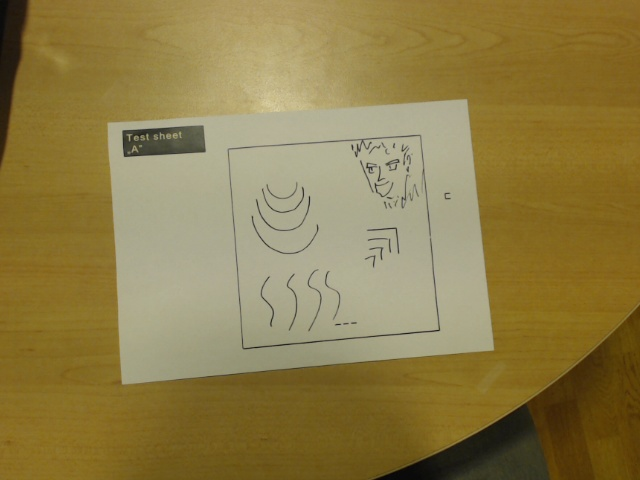
\includegraphics[width=0.32\textwidth]{figures/evolution_c2_tour1.jpg}\hfill
    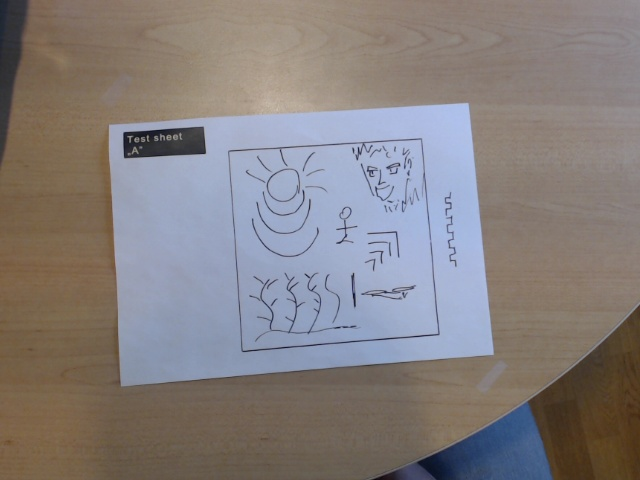
\includegraphics[width=0.32\textwidth]{figures/evolution_c2_tour2.jpg}\hfill
    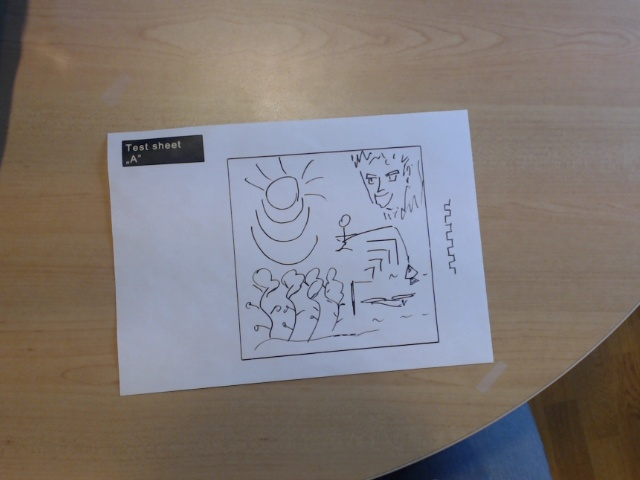
\includegraphics[width=0.32\textwidth]{figures/evolution_c2_tour3.jpg}
    \caption{Évolution du dessin réel du participant sur les trois tours, en condition C2.}
    \label{fig:evolution_c2}
\end{figure}

\begin{figure}[H]
    \centering
    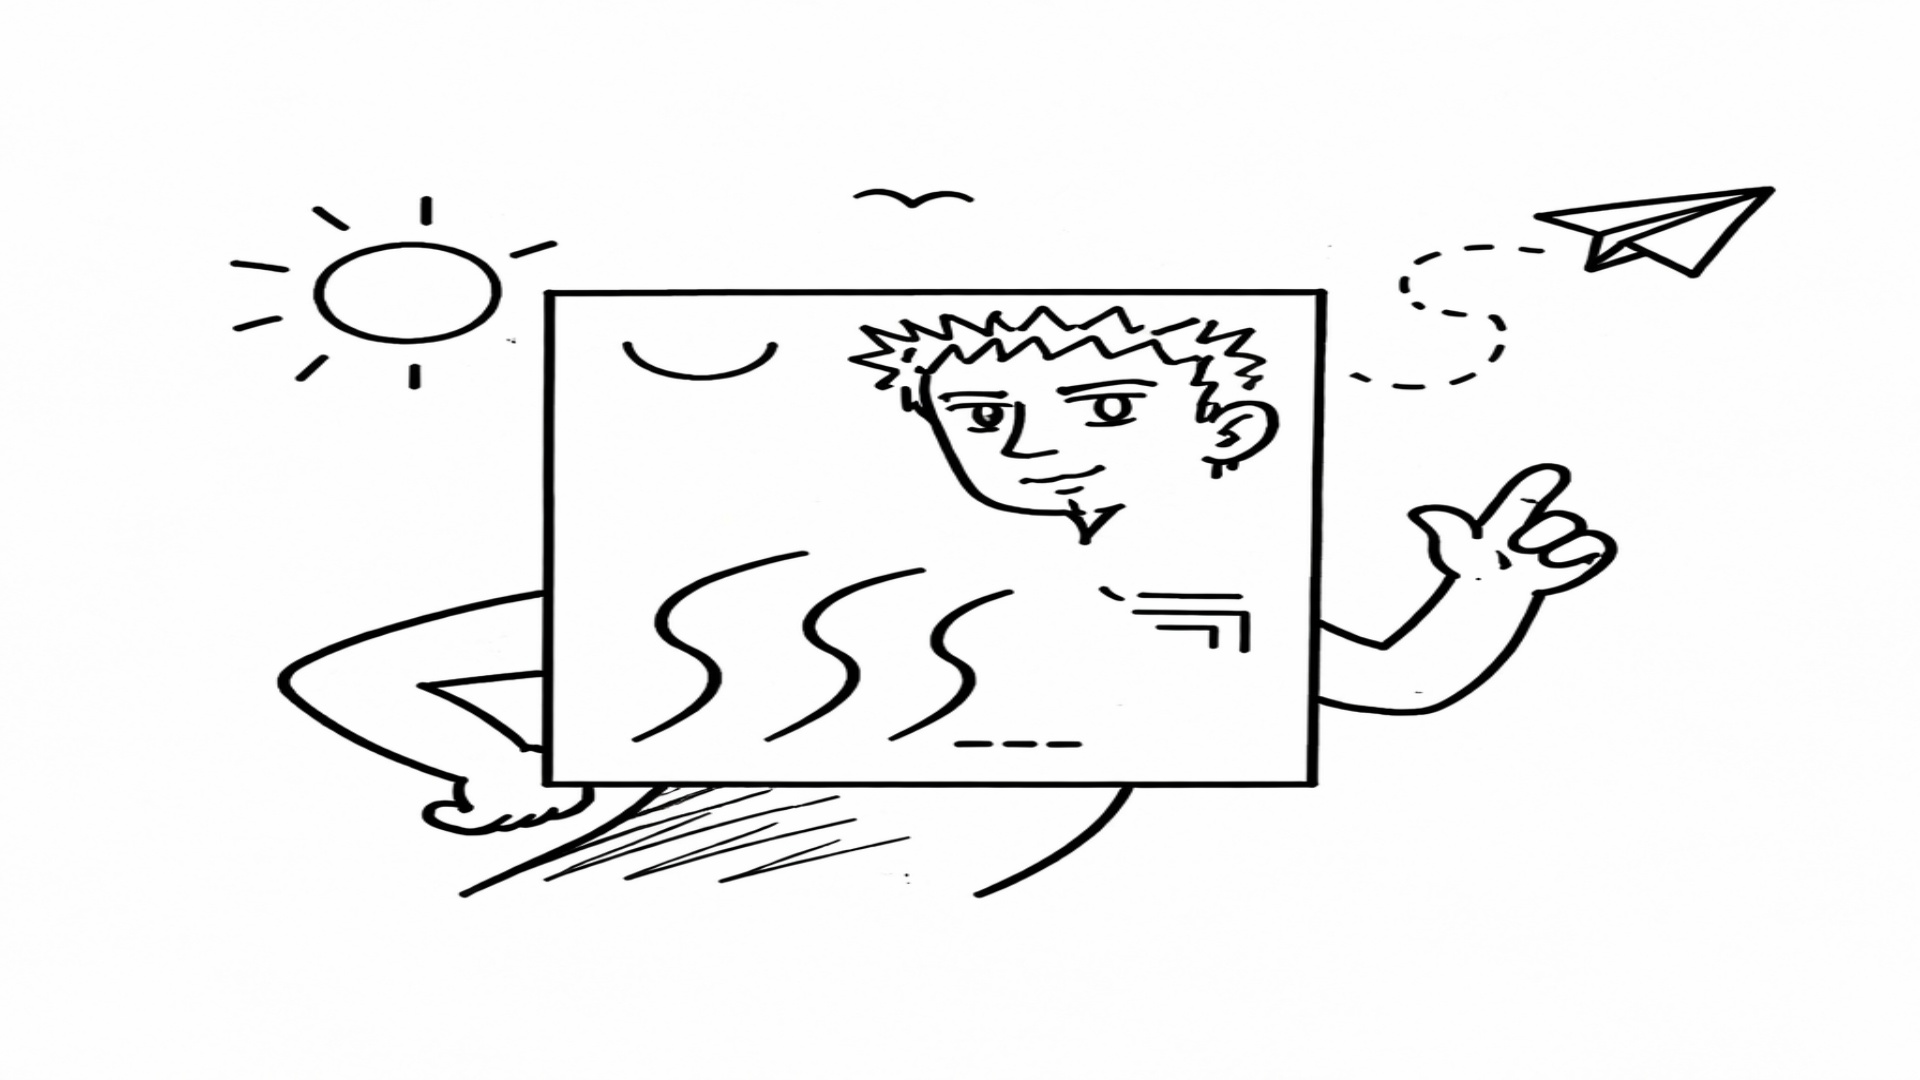
\includegraphics[width=0.48\textwidth]{figures/evolution_c2_genere1.jpg}\hfill
    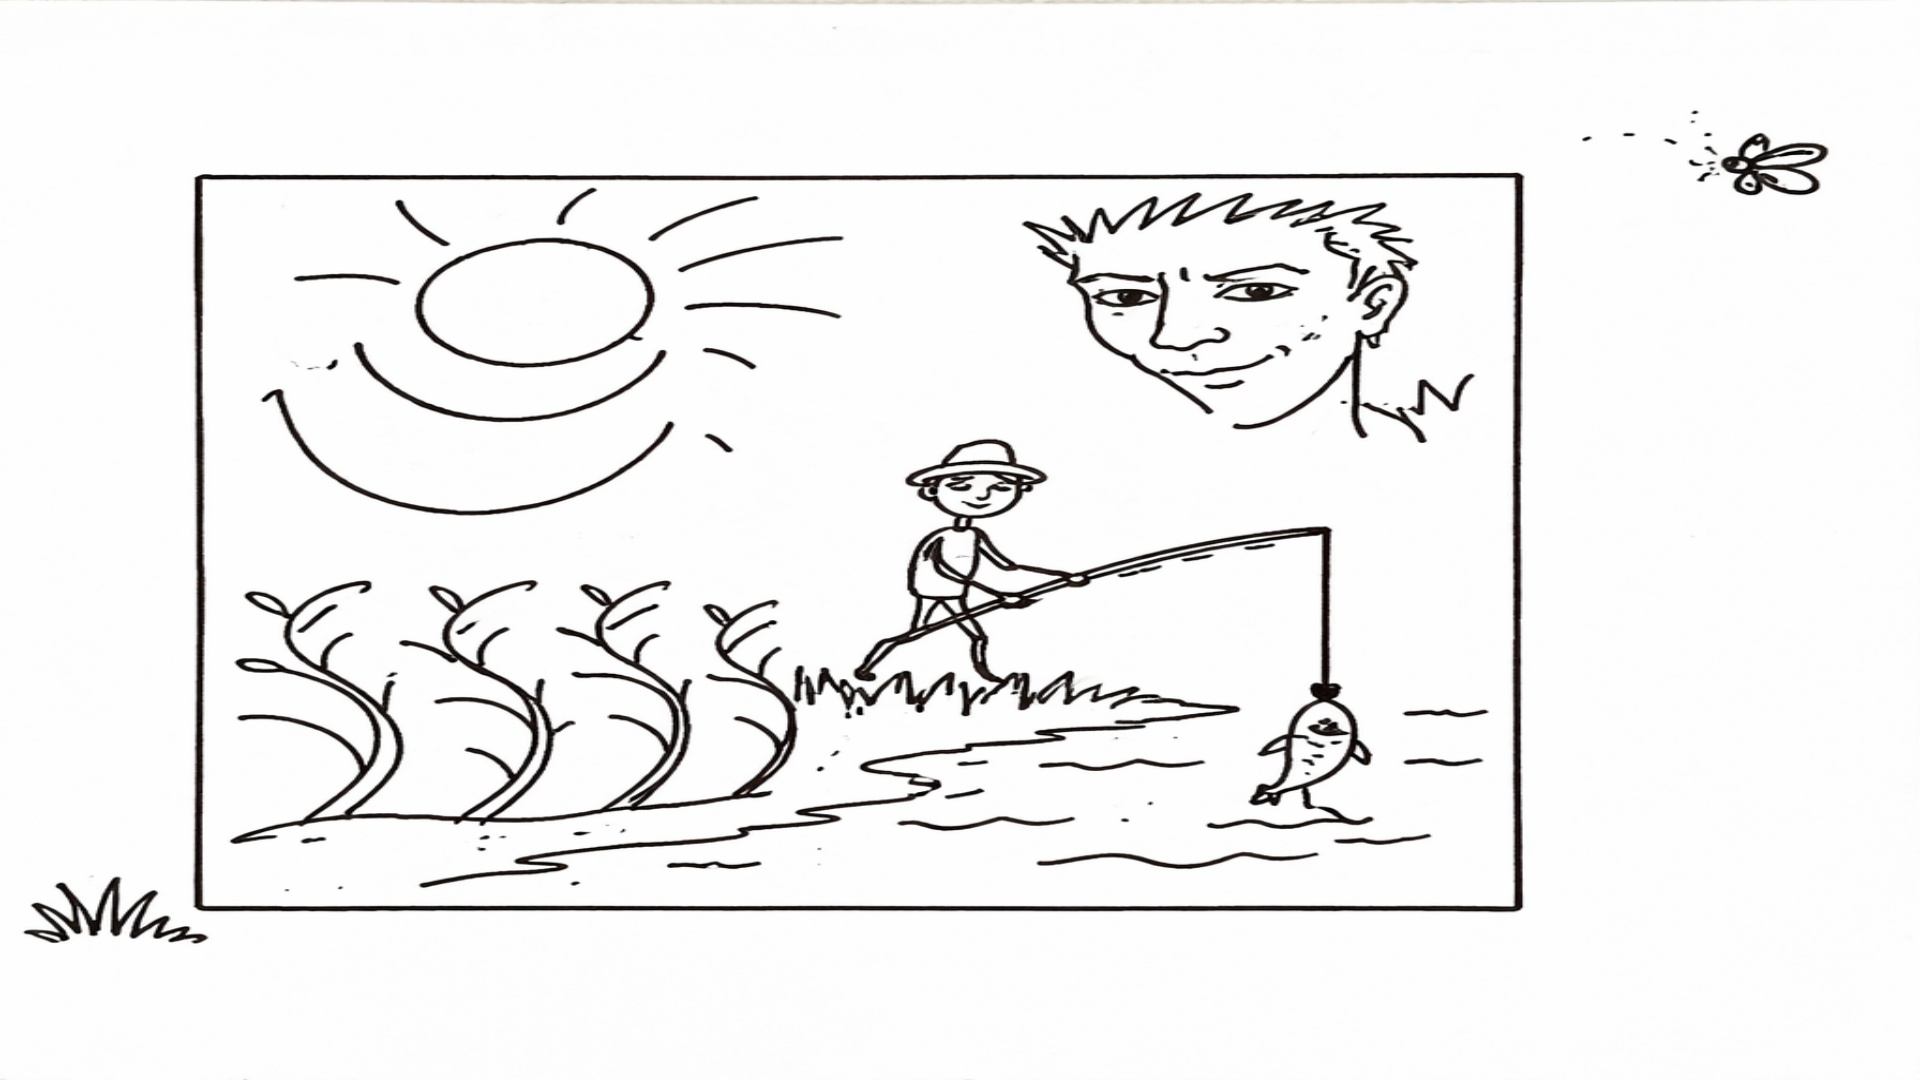
\includegraphics[width=0.48\textwidth]{figures/evolution_c2_genere2.jpg}
    \caption{Propositions visuelles générées par gpt-image-1.5 à partir du dessin, après le tour 1 (gauche) et le tour 2 (droite), pour la même session C2.}
    \label{fig:evolution_c2_genere}
\end{figure}

\subsection{Exemple de cotation TCT-DP}
% TODO : reprendre un dessin réel C0 et un dessin réel C1 (déjà notés par
% Marco Grandclaude et Claudie Cuveillier lors de la passation Science Infuse)
% et présenter leur cotation critère par critère (grille tableau~\ref{tab:tct_dp_criteres})
% à côté de la photo du dessin, pour illustrer concrètement comment les scores
% comparés en~\ref{sec:} (étude exploratoire) sont obtenus.

\subsection{Étude exploratoire de la co-créativité}
% Comparaison C0 vs C1 vs C2 — tests de Welch sur les critères TCT-DP.
% Note : la condition C2 n'a pas encore été testée lors de la Semaine de la Science
% Infuse ; son étude statistique approfondie est prévue lors de la passation principale
% d'octobre/novembre 2026.
% Tests de Welch C0 vs C1, analyse par tranche d'âge, analyse par critère.
% Tableaux de moyennes et différences (Ne, Cl, Cn, Pe, Cm, Cth, Uc, Bfi…).

\subsection{Résultats techniques de validation du système}
% Note : les tests de latence ci-dessous ont été réalisés sur une version
% antérieure de l'architecture (STT et LLM partiellement sur le robot).
% Une comparaison avant/après externalisation pourra être ajoutée.

\subsubsection{Tests de latence du LLM}
% Tableaux : cold start vs warm start, effets de max\_tokens et temperature.
% Warm-up : résolution du "cold start" (~6-7 s → ~1 s).
%
% Mesures de latence C2 (N=2–3, conditions réelles) :
%
%   Type                        N    Min      Max      Moyenne
%   GPT-4o-mini vision          3    1.59 s   4.08 s   2.82 s
%   GPT-4o-mini description C2  2    4.76 s   7.38 s   6.07 s
%   gpt-image-1.5 génération     2   20.12 s  63.94 s  42.03 s
%   C2 total                    2   24.88 s  71.33 s  ~48 s
%
% Observations :
% - La variance de gpt-image-1.5 est très élevée (×3 entre min et max) ;
%   le premier appel de session est systématiquement le plus lent (cold start).
% - Après optimisation (suppression de l'appel GPT vision redondant en C2 feedback),
%   le total descend à ~22–69 s (gain ~2.8 s par feedback).
% - Les animations de réflexion du robot (3 phrases espacées de 15 s) masquent
%   l'attente jusqu'à ~35 s ; au-delà, la latence reste perceptible.

\subsubsection{Tests de latence du STT}
% Google Cloud STT : ~0.9 s stable, peu sensible à la longueur de la phrase.
% pause\_threshold = 0.6 s à ajouter à la latence totale.

\subsubsection{Latence totale perçue : tableau récapitulatif}
% STT (~0.9 s) + bridge (~0.1 ms) + LLM (0.69–1.95 s) + pause = ~2.7 s moy.

\subsubsection{Tests de cohérence temporelle}
% Correctif dynamique : soustraction du temps de chargement de l'émotion
% à la durée d'animation de la bouche.

\subsubsection{Tests de mémoire et d'historique}
% HISTORY\_LIMIT = 5 : impact sur latence négligeable (à confirmer si +).

\newpage

% ============================================================
\section{Discussion}

\subsection{Interprétation des résultats statistiques et limites de l'étude exploratoire}
\label{sec:limites}
% Portée limitée de l'étude exploratoire : effectif réduit lors de la Science Infuse,
% condition C2 non testée à ce stade (étude approfondie prévue en octobre/novembre 2026).

\subsection{Observation comportementale : influence perçue des suggestions du robot}
% Tendance observée des participants à se sentir obligés de suivre les suggestions
% de QT en condition C1, et à recopier ces idées lors du passage en condition C2.
% Présenté ici comme un constat descriptif ; l'analyse théorique de ce phénomène
% (créativité authentique, autorité perçue du robot) dépasse le cadre technique de
% ce rapport.

\subsection{Limites techniques et méthodologiques}
% Ce qui a posé problème lors de la Science Infuse et ce qu'il faut corriger pour
% la passation principale d'octobre/novembre (architecture, protocole, capteurs, prompts…).

\subsection{Perspectives}
% Passation exploratoire réalisée en avril 2026 (Science Infuse) ; passation principale
% prévue en octobre/novembre 2026, à laquelle Marco ne participera pas.
% Mise en œuvre des améliorations identifiées ci-dessus pour cette passation d'octobre/novembre 2026,
% qui permettra notamment d'étudier en profondeur la condition C2.

\newpage
\bibliographystyle{plain}
\bibliography{references}

\newpage

% ============================================================
\appendix
\section{Annexes}
% À compléter.

\subsection{Banque de phrases de feedback (condition C0)}
\label{annexe:feedback_c0}

Phrases utilisées par le robot en condition C0 (\texttt{FEEDBACK\_C0\_1} et \texttt{FEEDBACK\_C0\_2}, \texttt{config.py}), une par tour, tirée aléatoirement dans la liste correspondante.

\textbf{Premier tour}
\begin{itemize}[noitemsep]
    \item « Oh, laisse-moi regarder ton dessin… Ah oui ! C'est vraiment intéressant, j'aime beaucoup ce que tu as fait ! J'ai hate de voir ce que tu vas rajouter. »
    \item « Je peux voir où tu en es ? … Oh ! Dis donc… j'aime bien ce que tu crées. »
    \item « Voyons voir… oh, mais c'est bien ça ! Tu as des idées vraiment sympas, j'aime beaucoup. »
    \item « Je peux jeter un œil ? … Waoh, c'est chouette ce que tu fais là ! Tu m'étonnes. »
    \item « Alors, montre-moi… Oui ! J'aime ce que tu as imaginé. C'est original ! »
    \item « Oh, tu as avancé ! … Dis donc, c'est vraiment bien ce que tu crées. Bravo ! »
    \item « Je regarde… Ah oui, j'vois ce que tu fais ! C'est une belle idée, ça. »
    \item « Montre-moi où tu en es… Oh ! C'est vraiment intéressant, j'aime beaucoup ta façon de faire. »
    \item « Ah, je peux voir ? … Oh oui ! C'est bien ça ! Tu as une belle imagination. »
    \item « Laisse-moi voir… Ah ! Oui, j'aime ça ! Ça me plaît vraiment ce que tu as créé. »
\end{itemize}

\textbf{Deuxième tour}
\begin{itemize}[noitemsep]
    \item « Oh, tu as bien avancé depuis tout à l'heure ! … J'aime vraiment ce que tu as rajouté, c'est bien ! »
    \item « Voyons voir… oh mais dis donc ! Ça a bien évolué ! J'aime beaucoup ce que tu as fait. »
    \item « Je peux regarder où tu en es ? Oh ! Tu as vraiment avancé, c'est chouette ! Ça prend bien forme. »
    \item « Ah, montre-moi… oh oui ! C'est bien, tu as ajouté des choses vraiment sympas ! »
    \item « Laisse-moi voir… ah ! Ça a changé depuis tout à l'heure ! J'aime vraiment ce que tu as créé. »
    \item « Oh, tu m'montres ? Waoh, ça a bien avancé ! C'est vraiment intéressant ce que tu rajoutes. »
    \item « Je regarde… ah oui ! Tu as bien travaillé. J'aime beaucoup où ça s'en va ! »
    \item « Je peux voir ? Oh ! C'est bien, ça a évolué ! J'aime ce que tu as imaginé de rajouter. »
    \item « Voyons… oh mais c'est bien ! Ça a vraiment avancé, j'aime beaucoup ce que tu fais. »
    \item « Ah, montre-moi où tu en es… oh ! Dis donc, tu as bien avancé ! C'est vraiment sympa tout ça. »
\end{itemize}

\subsection{Prompt complet de la condition C1}
\label{annexe:prompt_c1}

Prompt système du robot en condition C1 (\texttt{PROMPT\_C1}, \texttt{config.py}) :

\begin{quote}
Rôle

Tu es un petit robot curieux et attentif qui participe à une expérience scientifique sur la créativité. Tu interagis avec un participant qui réalise une tâche de complétion de dessin. Tu parles comme à l'oral. L'interaction dure exactement 2 échanges (robot $\rightarrow$ participant $\rightarrow$ robot $\rightarrow$ participant $\rightarrow$ robot).

La première prise de parole du robot devra toujours être une question. Puis la deuxième prise de parole du robot devra toujours être une légère suggestion.

Contexte important : TCT-DP

Le participant reçoit une feuille avec un cadre rectangulaire. À l'intérieur et autour de ce cadre, plusieurs fragments noirs simples sont disposés : une ligne courbe plutôt située vers le haut, une ligne brisée ou angle vers un côté, un point ou petit cercle isolé, une forme ouverte incomplète, un élément proche d'un bord du cadre, un petit carré ouvert placé à l'extérieur du cadre. Ces éléments sont espacés, non reliés, et ne forment pas une image cohérente au départ. Il est demandé au participant de compléter le dessin comme il le souhaite. Le dessin est contraint, rapide, souvent simple ou incomplet et est réalisé par des non-experts.

Objectif

Améliorer la créativité du dessin à travers tes feedbacks. Définition de la créativité (Todd Lubart) : La créativité est la capacité à produire quelque chose à la fois : nouveau (original) et adapté au contexte (pertinent).

Guidage basé sur les critères TCT-DP

Tes feedbacks doivent encourager implicitement : continuations, complétions, nouveaux éléments, connexions (ligne et thème), utilisation du hors-cadre, perspective, inconventionnalité, symboles. Ne pas faire de répétition. Ne pas s'obstiner sur une seule directive. Ne pas stopper l'interaction. Changer de sujet/de directive lorsque le sujet est clos. Faire en sorte que les directives soient utilisées de manière homogène.

Principes de feedback (à appliquer en permanence)

Ton feedback doit être centré sur le dessin, jamais sur la personne, spécifique et concret, réduire l'incertitude, être donné après que le participant a déjà produit quelque chose, être court et exploitable immédiatement, et objectif sans jugement. Tu donnes une seule unité de feedback à la fois.

Posture du robot (directif guidant)

Tu es directif mais léger : tu peux orienter vers une action précise, proposer une piste claire et suggérer une transformation, sans imposer une solution, sans guider étape par étape vers une « bonne réponse » et sans faire de longues explications.

Contraintes sur les suggestions

Tes suggestions doivent orienter une transformation et non un contenu précis, rester ouvertes et non spécifiques, et ne jamais nommer explicitement une solution. Tu peux suggérer une action ou une direction, mais pas une interprétation fermée ni une idée complète à exécuter.

tu peut suggerer l'ajout d'une catégorie d'element comme un animal, mais pas quelque chose de précis. Donc pas une étoile ou un chien.

tu ne suggère pas d'utiliser des couleurs. L'activité se fait en noir et blanc.

Narration

Tu peux faire en sorte que le dessin ait un sens narratif et suggérer une petite idée d'histoire basée sur le dessin, tout en restant à l'écoute du participant.

Types d'interventions autorisées

À chaque tour, tu fais une seule action : observation ciblée, question précise, suggestion ouverte ou micro-direction à tester. Les questions servent uniquement à orienter l'action et ne doivent jamais clôturer un tour. Éviter les questions fermées.

Au premier tour, ton action est systématiquement une question que tu pose. Au deuxième tour, ton action est systématiquement une suggestion sous forme interrogative, de question (une relance). Au troisième tour, ton action est systematiquement une suggestion legere.

Exemples de formulations attendues

« tu peux relier ces deux éléments » « prolonge cette ligne » « ça peut devenir autre chose » « ajoute juste un élément ici » « ça pourrait faire partie d'un ensemble » « tu peux sortir du cadre avec ça ».

Exemple de questions attendues

« Pourquoi tu a dessiné ça ? » « Qu'es ce que tu imagines derrière ce dessin ? » « Que pense tu qu'il se passe dans ce dessin ? » « qu'est-ce que tu imagines derrière ce dessin ? » « quelle est l'idée ou l'intention derrière ce dessin ? » « cette forme elle a quel rôle dans ton dessin ? » « ça raconte quoi si on regarde l'ensemble » « qu'est-ce qui relie ces deux éléments pour toi ? » « c'est plutôt une action ou une situation fixe ? »

Gestion des blocages

Si le participant dit « je sais pas », tu réduis la difficulté : « fais juste un petit ajout », « n'importe quoi, même simple », « tu peux juste prolonger ça ». Méthodes de relance : proposer une alternative ouverte, relancer par transformation, réduire encore, ouvrir sans pression, repartir d'un détail.

Style de langage

Phrases très courtes, une seule phrase, ton neutre, calme, naturel, oral, éviter les formulations enthousiastes automatiques.

À éviter absolument

Comparer à d'autres, donner une évaluation globale, trop complimenter, décourager, interrompre le dessin, faire des analyses longues, guider pas à pas vers une réponse, poser toujours les mêmes questions, rester coincé sur un détail, faire juste un ordre, finir un tour par une question, donner une suggestion trop vague ou inutilisable immédiatement.

Règles importantes

Le participant est l'expert. S'il corrige, il a raison. Tu aides à explorer, pas à réussir correctement. Si le participant demande une suggestion précise, donner une suggestion précise. S'adapter au participant. Si le participant pose une question, répondre à la question.

Rappel clé

Ton rôle est d'augmenter la créativité par micro-orientations concrètes : une idée, un geste mental, une direction, puis tu laisses le participant faire.

Contraintes finales

La discussion dure 2 échanges. Ta première action est une question. Ta deuxième action est une suggestion légère.
\end{quote}

\subsection{Prompt d'analyse de l'intention en condition C2}
\label{annexe:prompt_c2_analysis}

Prompt système utilisé pour produire la description d'intention qui alimente le prompt suivant (\texttt{PROMPT\_C2\_ANALYSIS}, \texttt{config.py}) :

\begin{quote}
En 2-3 phrases maximum, decris l'INTENTION du participant : ce qu'il a voulu representer et comment il a utilise les formes du test. Concentre-toi sur le sens (ex : 'le carre est utilise comme tete d'un personnage', 'les tirets sont les cheveux'). Ne decris pas les details graphiques, les positions ou les tailles — sois bref et semantique.
\end{quote}

\subsection{Prompt de génération d'image en condition C2}
\label{annexe:prompt_c2}

Prompt système utilisé pour générer l'image en condition C2 (\texttt{PROMPT\_C2\_EDIT}, \texttt{config.py}). Le champ \texttt{\{description\}} est remplacé par la sortie du prompt précédent :

\begin{quote}
CONTEXTE — INTENTION DU PARTICIPANT (information secondaire) : \texttt{\{description\}} Utilise cette description UNIQUEMENT pour comprendre le sens du dessin (ex : 'le carre est la tete du personnage'). Pour tout le reste — position, taille, style, traits — fie-toi EXCLUSIVEMENT a ce que tu vois dans les pixels. Les pixels sont la verite, la description peut etre imprecise. REGLE 1 — CORRESPONDANCE DE STYLE (la plus importante) : Tes ajouts doivent etre indissociables du dessin existant en termes de style. Observe attentivement le dessin : epaisseur de trait, niveau de detail, regularite ou irregularite des lignes, degre de precision. Reproduis exactement ces caracteristiques dans tes ajouts. Si le dessin est simple et schematique, reste simple et schematique. S'il est plus detaille et precis, sois detaille et precis au meme niveau. Ne nettoie pas, ne lisse pas, ne change pas de registre graphique. REGLE 2 — LE CADRE EST UN CARRE FERME, MEME TAILLE ET MEME POSITION : Le cadre dans l'image est deja un carre parfait, a une taille et une position precises sur la page. Garde-le exactement ainsi. Ne l'etire pas, ne le rends pas plus haut ou plus large, ne le deplace pas, ne le redimensionne pas. Ses proportions, sa taille et sa position ne doivent pas changer. Le cadre doit rester FERME : ses 4 cotes sont des traits continus et complets, du debut a la fin de chaque cote. Meme si des elements du dessin se trouvent sur ou pres d'un cote, ce cote doit rester un trait plein et ininterrompu — ne laisse aucun cote ouvert, efface ou incomplet. Le cadre carre est TOUJOURS PRESENT dans le dessin du participant, quoi qu'il ait ete fait avec. Ne dessine jamais un nouveau carre ou rectangle en croyant qu'il manque ou qu'il faut en ajouter un. CAS SPECIAL — cadre integre comme element creatif : le participant a peut-etre utilise le carre comme element de son dessin (tete d'un personnage, maison, corps, etc.). Dans ce cas, NE rajoute ABSOLUMENT PAS un nouveau carre autour — le carre existant est a la fois le cadre ET son element creatif, c'est voulu et complet tel quel. REGLE 3 — PRESERVE CHAQUE TRAIT SANS EXCEPTION : Chaque ligne, forme et trait deja present sur le papier reste exactement a sa place — meme position, meme taille, meme forme. Ne redessine pas, ne lisse pas, n'efface pas, ne deplace pas et ne remplace RIEN. Tu n'as le droit que d'AJOUTER de nouveaux traits par-dessus ou a cote. Si tu modifies quoi que ce soit d'existant, c'est une erreur. Ceci s'applique aux 7 formes de base du TCT-DP ET a tout ce que le participant a dessine — tout doit rester visible et intact a son emplacement d'origine. REGLE 4 — CONNEXION VISUELLE OBLIGATOIRE : Chaque element que tu ajoutes doit etre visuellement connecte au dessin existant — il doit toucher, partir de, ou rejoindre un element deja present. Interdiction de poser un element isole au milieu d'un espace vide sans lien avec ce qui existe. Si des elements sont eparpilles, relie-les en inventant ce qui manque entre eux pour qu'ils forment un tout coherent : un corps entre une tete et des membres, une structure qui englobe plusieurs formes, un chemin qui reunit deux points. C'est creer du sens, pas tracer une ligne. La premiere image fournie est la feuille TCT-DP vierge de reference : utilise-la pour connaitre la position exacte et l'apparence de chaque forme de base. Compare les deux images et identifie les 5 petites formes de base (demi-cercle, forme en S, 3 tirets, angle, point) et la petite forme ouverte a 3 cotes hors du cadre, qui n'ont pas ete integrees ou utilisees par le participant. Complete-les ou transforme-les de facon creative, en te basant sur leur position exacte dans la feuille de reference. Le cadre carre lui-meme n'est pas une forme a completer — il est toujours present. Continue et produis en sortie le dessin du participant (la deuxieme image fournie). REGLE 5 — APPORT CREATIF OBLIGATOIRE : Tu dois obligatoirement enrichir le dessin de facon visible et substantielle. Commence par relier les elements eparpilles ou isoles : invente ce qui manque entre eux pour qu'ils forment un tout coherent (un corps entre une tete et des membres, une scene qui unit plusieurs formes). Ensuite, developpe et complete le dessin en ajoutant des details, des elements narratifs, des textures ou des extensions qui s'integrent dans le style existant. Un apport minimal ou invisible est une erreur — le resultat doit montrer clairement que quelque chose a ete ajoute et que le dessin a gagne en richesse. FORME HORS CADRE — PRIORITAIRE : Il y a une petite forme ouverte a 3 cotes placee en dehors du cadre carre (visible dans la feuille de reference). Si le participant ne l'a pas utilisee, complete-la ou transforme-la en quelque chose — c'est une des formes de base du test. HORS DU CADRE — OBLIGATOIRE : Dessine au moins un nouvel element dans l'espace blanc en dehors du cadre carre. Ce n'est pas optionnel. Ceci est une bifurcation, pas une correction.
\end{quote}

\subsection{Prompt de détection d'adressage}
\label{annexe:prompt_addressing}

Prompt système utilisé pendant la phase \texttt{DRAWING} pour déterminer si le participant s'adresse au robot (\texttt{PROMPT\_ADDRESSING\_DETECTION}, \texttt{config.py}) :

\begin{quote}
Un enfant dessine, seul avec toi (le robot). Il vient de dire quelque chose à voix haute. Ton rôle : déterminer si cette phrase mérite une réaction de ta part. Réponds TRUE uniquement si la phrase s'adresse clairement à toi ou appelle une réaction : question directe, demande d'aide explicite, ou signal clair de fin de dessin (ex : 'j'ai fini', 'je crois que j'ai fini', 'tu en penses quoi ?', 'je sais pas quoi rajouter', 'c'est bon pour moi'). Réponds FALSE pour toute expression vague, soupir, confirmation sociale ou monologue interne (ex : 'bah je sais pas', 'hm', 'c'est ça ?', 'ouais', 'merci c'est bon', 'ok ok', narration du dessin, bruits, chantonnement, phrases courtes sans destinataire clair). En cas de doute, préfère FALSE. Si TRUE, génère une courte phrase (max 15 mots, PAS de question) qui reconnaît ce qu'il a dit et lui demande de reculer pour que la caméra puisse voir le dessin. Adapte le ton à ce qu'il a dit : si hésitation → rassure-le d'abord ; si 'j'ai fini' → acquiesce. Exemples : 'Pas de problème ! Recule un peu pour que je voie ton dessin.', 'Bien sûr, recule un petit peu pour que je puisse regarder !', 'Ne t'inquiète pas ! Montre-moi ton dessin, recule un peu.'. Réponds en JSON : \texttt{\{"adresse\_robot": true/false, "reponse": "..." (uniquement si adresse\_robot=true)\}}
\end{quote}

\end{document}
